\documentclass[10pt]{beamer}
\usetheme[
%%% option passed to the outer theme
%    progressstyle=fixedCircCnt,   % fixedCircCnt, movingCircCnt (moving is deault)
  ]{Berlin}
  
% If you want to change the colors of the various elements in the theme, edit and uncomment the following lines

% Change the bar colors:
%\setbeamercolor{Feather}{fg=red!20,bg=red}

% Change the color of the structural elements:
%\setbeamercolor{structure}{fg=red}

% Change the frame title text color:
%\setbeamercolor{frametitle}{fg=blue}

% Change the normal text color background:
%\setbeamercolor{normal text}{fg=black,bg=gray!10}

%-------------------------------------------------------
% INCLUDE PACKAGES
%-------------------------------------------------------

\usepackage[utf8]{inputenc}
\usepackage[english]{babel}
\usepackage[T1]{fontenc}
\usepackage{amsmath}
\usepackage{helvet}
\usepackage{multirow}
\usepackage{graphicx}
\usepackage{comment}
\usepackage[absolute,overlay]{textpos}
\usepackage{tabularx}
\usepackage{tikz}
\usetikzlibrary{arrows,automata,positioning}
\usetikzlibrary{shapes.multipart}
\usetikzlibrary{decorations.markings}
\usetikzlibrary{matrix}
\usepackage{marvosym}
\usepackage[marvosym]{tikzsymbols}

%-------------------------------------------------------
% DEFFINING AND REDEFINING COMMANDS
%-------------------------------------------------------

% colored hyperlinks
%\renewcommand*{\Footnotemark}[1]{\NCC@makefnmark{#1}}
\newcommand{\chref}[2]{
  \href{#1}{{\usebeamercolor[bg]{Feather}#2}}
}
\newcommand{\tuple}[1]{{\langle #1 \rangle}}
\newcommand{\pre}{\mathsf{pre}}     % precondition
\newcommand{\eff}{\mathsf{eff}}     % effect
\newcommand{\cond}{\mathsf{cond}}   % conditional effect

\newcommand{\X}{\mathcal{X}}
\newcommand{\F}{\mathcal{F}}
\newcommand{\A}{\mathcal{A}}
\newcommand{\N}{\mathcal{N}}
\newcommand{\I}{\mathcal{I}}
\newcommand{\real}{\mathbb{R}}
\newcommand{\Dw}{\mathcal{D}}
\newcommand{\Xw}{\mathcal{X}}
\newcommand{\Aw}{\mathcal{A}}
\newcommand{\Rw}{\mathcal{R}}
\newcommand{\OO}{\mathcal{O}}
\newcommand{\tOO}{\wt{\OO}}
\newcommand{\II}[1]{\mathbb{I}{\left\{#1\right\}}}
\newcommand{\PP}[1]{\mathbb{P}\left[#1\right]}
\newcommand{\EE}[1]{\mathbb{E}\left[#1\right]}
\newcommand{\EEs}[2]{\mathbb{E}_{#2}\left[#1\right]}
\newcommand{\PPt}[1]{\mathbb{P}_t\left[#1\right]}
\newcommand{\EEt}[1]{\mathbb{E}_t\left[#1\right]}
\newcommand{\PPi}[1]{\mathbb{P}_i\left[#1\right]}
\newcommand{\EEi}[1]{\mathbb{E}_i\left[#1\right]}
\newcommand{\EEp}[1]{\mathbb{E}_{\pi,P}\left[#1\right]}
\newcommand{\EEcp}[2]{\mathbb{E}_{\pi,P}\left[\left.#1\right|#2\right]}
\newcommand{\PPc}[2]{\mathbb{P}\left[#1\left|#2\right.\right]}
\newcommand{\PPct}[2]{\mathbb{P}_t\left[#1\left|#2\right.\right]}
\newcommand{\PPcc}[2]{\mathbb{P}\left[\left.#1\right|#2\right]}
\newcommand{\PPcct}[2]{\mathbb{P}_t\left[\left.#1\right|#2\right]}
\newcommand{\PPcci}[2]{\mathbb{P}_i\left[\left.#1\right|#2\right]}
\newcommand{\EEc}[2]{\mathbb{E}\left[#1\left|#2\right.\right]}
\newcommand{\EEcc}[2]{\mathbb{E}\left[\left.#1\right|#2\right]}
\newcommand{\EEcs}[3]{\mathbb{E}_{#3}\left[\left.#1\right|#2\right]}
\newcommand{\EEcct}[2]{\mathbb{E}_t\left[\left.#1\right|#2\right]}
\newcommand{\EEcci}[2]{\mathbb{E}_i\left[\left.#1\right|#2\right]}
\renewcommand{\th}{\ensuremath{^{\mathrm{th}}}}
\def\argmin{\mathop{\mbox{ arg\,min}}}
\def\argmax{\mathop{\mbox{ arg\,max}}}
\newcommand{\ra}{\rightarrow}

\newcommand{\norm}[1]{\left\|#1\right\|}
\newcommand{\onenorm}[1]{\norm{#1}_1}
\newcommand{\infnorm}[1]{\norm{#1}_\infty}
\newcommand{\iprod}[2]{\left\langle#1,#2\right\rangle}
\newcommand{\ev}[1]{\left\{#1\right\}}
\newcommand{\pa}[1]{\left(#1\right)}
\newcommand{\bpa}[1]{\bigl(#1\bigr)}
\newcommand{\Bpa}[1]{\Bigl(#1\Bigr)}
\newcommand{\sign}{\mbox{sign}}
\newcommand{\wh}{\widehat}
\newcommand{\wt}{\widetilde}
\newcommand{\transpose}{^\top}

\newcommand{\loss}{\ell}
\newcommand{\hloss}{\wh{\loss}}
\newcommand{\hL}{\wh{L}}
\newcommand{\tZ}{\wt{Z}}
\newcommand{\reg}{\mathfrak{R}}
\newcommand{\hreg}{\widehat{\reg}}
\newcommand{\hr}{\wh{r}}
\newcommand{\hv}{\wh{v}}
\newcommand{\hq}{\wh{q}}
\newcommand{\hmu}{\wh{\mu}}
\newcommand{\hR}{\wh{R}}
\newcommand{\tmu}{\wt{\mu}}
\newcommand{\tN}{\wt{N}}
\newcommand{\RE}[2]{\mbox{RE}\left(\left.#1\right\|#2\right)}
\newcommand{\KL}[2]{\mbox{KL}\left(#1\middle\lVert#2\right)}
\newcommand{\DD}[3]{D_{#3}\left(#1\middle\lVert#2\right)}
\newcommand{\DDC}[2]{\DD{#1}{#2}{C}}
\newcommand{\DDS}[2]{\DD{#1}{#2}{S}}

\newcommand{\trho}{\wt{\rho}}

\definecolor{gold}{rgb}{1,0.75,0}
\definecolor{darkred}{rgb}{0.75,0,0}
\setbeamercolor*{goldc}{fg=black,bg=gold}
\definecolor{darkpurp}{rgb}{0.4,0.2,0.4}
\setbeamercolor*{purpc}{fg=white,bg=darkpurp}
\setbeamercolor*{redc}{fg=white,bg=darkred}
\newcommand{\hG}[1]{\large \textcolor{darkred}{#1}}

\newcommand{\redd}[1]{\textcolor{darkred}{#1}}
\newcommand{\goldd}[1]{\textcolor{gold}{#1}}

\definecolor{ballblue}{rgb}{0.0, 0.5, 0.5}
\definecolor{lightgray}{rgb}{0.85, 0.85, 0.85}

%-------------------------------------------------------
% INFORMATION IN THE TITLE PAGE
%-------------------------------------------------------

\title[] % [] is optional - is placed on the bottom of the sidebar on every slide
{ % is placed on the title page
      \textbf{Machine Learning}
}

\author[Jonsson \& G\'omez]
{      Anders Jonsson \& Vicen\c{c} G\'omez \\
\vspace*{0.5cm}
Master in Intelligence Interactive Systems\\
2021-22\\
\vspace*{0.5cm}
Lecture 7\\
Deep learning
%      {\ttfamily bagchi.bhaskar@cse.iitkgp.ernet.in}
}

\date{}

\AtBeginSection[]
{
   \begin{frame}
       \frametitle{Content}
       \tableofcontents[currentsection]
   \end{frame}
}

%-------------------------------------------------------
% THE BODY OF THE PRESENTATION
%-------------------------------------------------------

\begin{document}

%-------------------------------------------------------
% THE TITLEPAGE
%-------------------------------------------------------

\begin{frame}[plain,noframenumbering] % the plain option removes the header from the title page, noframenumbering removes the numbering of this frame only
  \titlepage % call the title page information from above
\end{frame}

\begin{frame}
    \tableofcontents
\end{frame}

\section{History of deep learning}

\begin{frame}
  \frametitle{History of deep learning}
  \begin{itemize}
	\item[1943] Computer model of artificial neuron [McCulloch and Pitts]
	\item[1960-70] Backpropagation algorithm for training neural networks [Kelley; Bryson; Dreyfus; Ivakhnenko; Lapa; Werbos]
	\item[1970-80] First AI winter
	\item[1980-86] Modern version of backpropagation [Linnainmaa; Fukushima; Parker; Rumelhart et al.]
	\item[1986-95] Second AI winter
	\item[1995-] Novel network models, faster processors, GPUs
	\item[2010-] Breakthrough of deep learning
  \end{itemize}
\end{frame}

\begin{frame}
\frametitle{Computational power}
\centerline{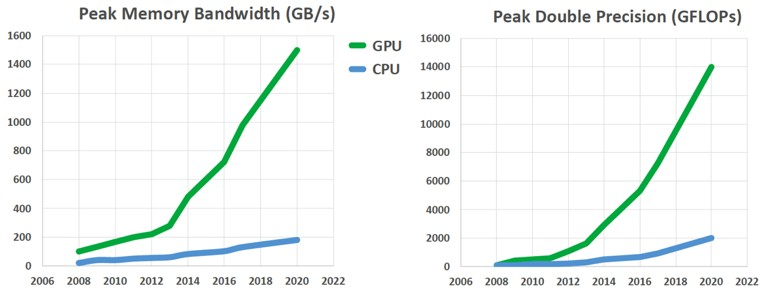
\includegraphics[height=5cm]{images/decade-gpu-natoli.jpg}}
\end{frame}

\begin{frame}
\frametitle{Supply and demand of data (2009-2020)}
\centerline{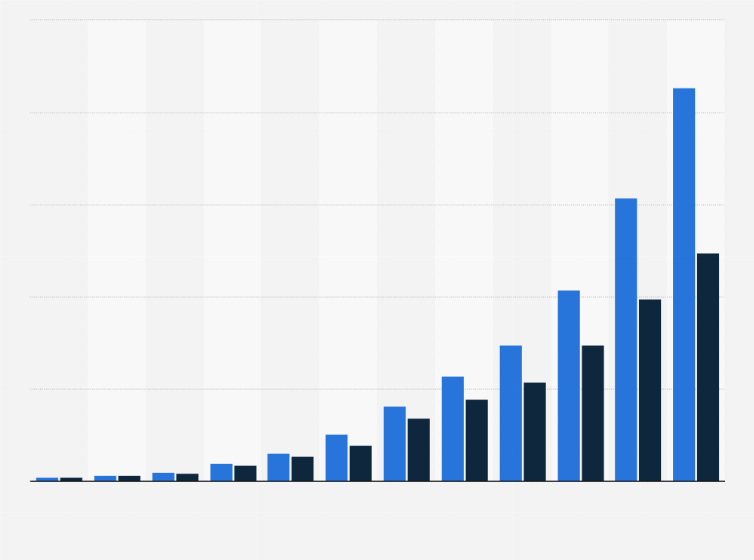
\includegraphics[height=6.5cm]{images/data.png}}
\end{frame}

\begin{frame}
\frametitle{Progress in image classification}
\centerline{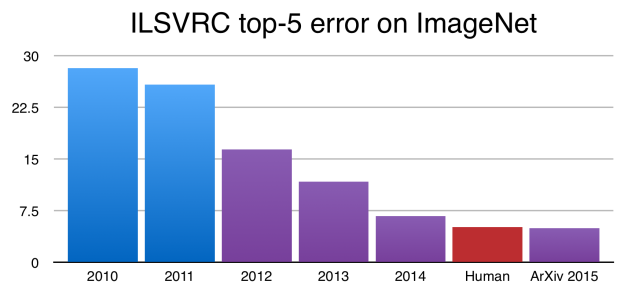
\includegraphics[height=4.5cm]{images/images_alt.png}}
\end{frame}

\section{Feedforward neural networks}

\begin{frame}
  \frametitle{Neuron}
  \begin{center}
  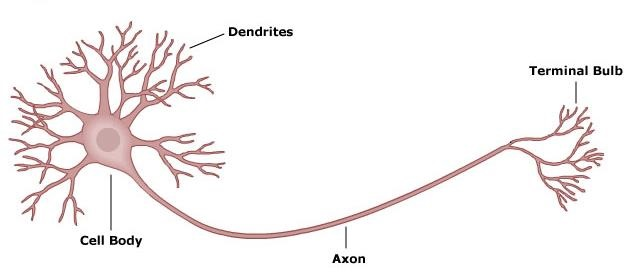
\includegraphics[height=5cm]{images/neuron.jpg}
  \end{center}
\end{frame}

\begin{frame}
\frametitle{Artificial neuron (McCulloch and Pitts, 1943)}
	\begin{center}
	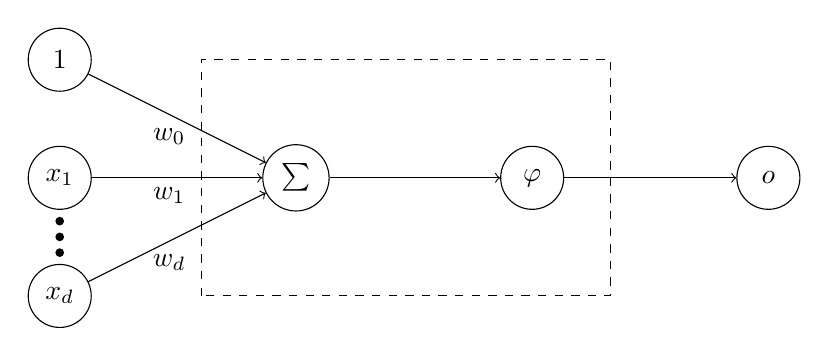
\begin{tikzpicture}
    \node[draw,circle,minimum size=.8cm] at (.8,3.3)  (a) {$1$};
    \node[draw,circle,minimum size=.8cm] at (.8,1.8)  (b) {$x_1$};
	\node[draw,circle,minimum size=.8cm] at (.8,.3)   (c) {$x_d$};
    \node[draw,circle,minimum size=.8cm] at (3.8,1.8) (d) {$\sum$};
    \node[draw,circle,minimum size=.8cm] at (6.8,1.8) (e) {$\varphi$};
    \node[draw,circle,minimum size=.8cm] at (9.8,1.8) (f) {$o$};

	\draw[thick,fill=black] (.8,1.25) circle (0.04cm);
	\draw[thick,fill=black] (.8,1.05) circle (0.04cm);
	\draw[thick,fill=black] (.8,0.85) circle (0.04cm);

    \draw[->] (a) -- (d) node[midway,below,xshift=-.1cm] {$w_0$};
    \draw[->] (b) -- (d) node[midway,below,xshift=-.1cm] {$w_1$};
    \draw[->] (c) -- (d) node[midway,below,xshift=-.1cm,yshift=-.1cm] {$w_d$};
    \draw[->] (d) -- (e);
    \draw[->] (e) -- (f);

	\draw[dashed] (2.6,.3) rectangle (7.8,3.3);
	\end{tikzpicture}
	\end{center}
\begin{itemize}
\item $x_1,\ldots,x_d$: inputs
\item $w_0,\ldots,w_d$: weights
\item $\varphi$: (non-linear) activation function
\item $o=\varphi(\sum_iw_ix_i)$: output
\end{itemize}
\end{frame}

\begin{frame}
\frametitle{Common activation functions}
\begin{tabular}{cc}
Classification & Regression\\[10pt]
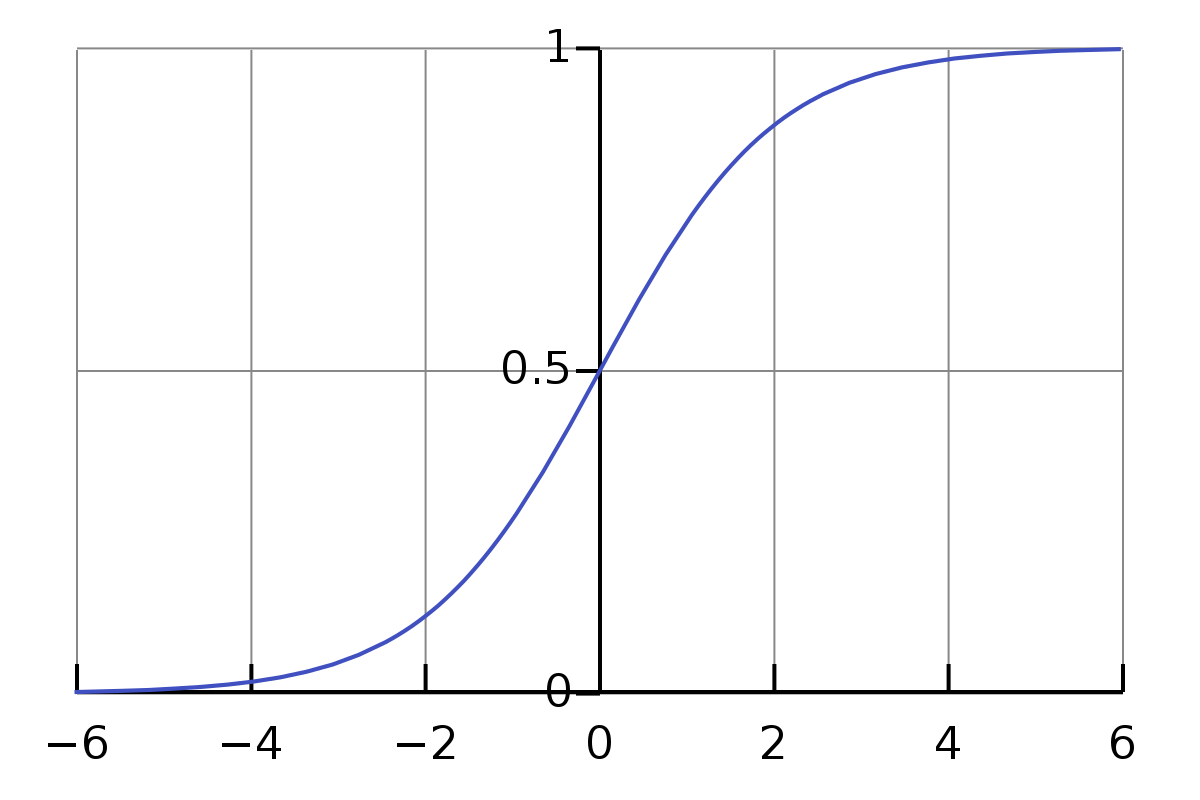
\includegraphics[height=3cm]{images/sigmoid.png} & 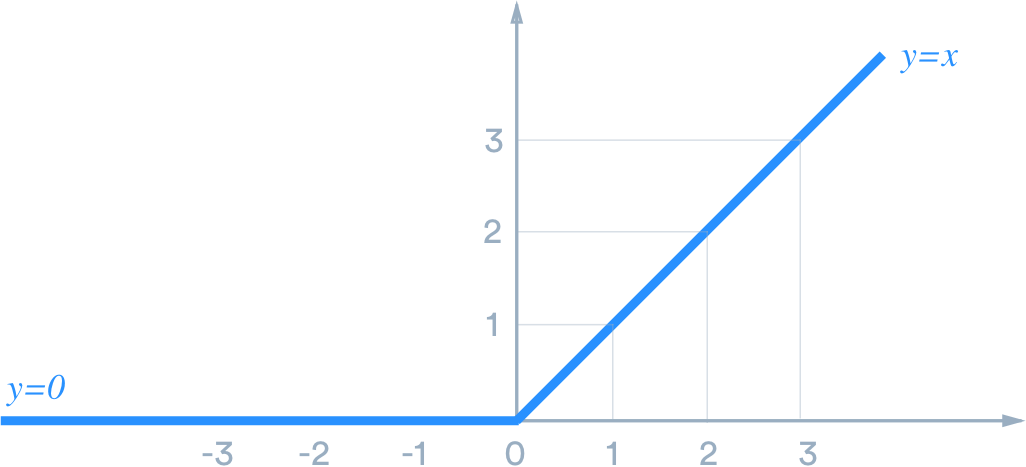
\includegraphics[height=2.5cm]{images/relu.png}\\[10pt]
Logistic function & Rectified Linear Unit (ReLU)\\[10pt]
$\varphi(s)=\frac{1}{1+e^{-s}}$ & $\varphi(s)=\max(0,s)$
\end{tabular}
\end{frame}

\begin{frame}
\frametitle{Input representation}
\begin{itemize}
\item {\color{red} Problem}: Neurons cannot handle categorical inputs
\item {\color{green} One-hot encoding}: represent categories as elements in a vector
\end{itemize}

\vspace*{1cm}

\begin{center}
  \begin{tikzpicture}[overlay]
	\node at (0,0) {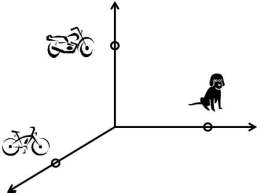
\includegraphics[height=3cm]{images/onehot.png}};
	\node at ( 1.2,-0.8) {$[1,0,0]$};
	\node at ( 0.5, 0.8) {$[0,1,0]$};
	\node at (-0.5,-1.3) {$[0,0,1]$};
  \end{tikzpicture}
\end{center}
\end{frame}

\begin{frame}
\frametitle{Vectorization}
\[\sum_{i=0}^d w_ix_i \;\; \Rightarrow \;\; {\bf w}^T{\bf x}\]
\begin{itemize}
\item For loops are {\color{red} inefficient}
\begin{itemize}
\item Hardware limitations
\item Programming language of choice
\end{itemize}
\item Instead, rewrite implementation using {\color{green} vector operations}
\begin{itemize}
\item Very fast in some programming languages (Python, Matlab)
\end{itemize}
\end{itemize}
\end{frame}

\begin{frame}
\frametitle{Feedforward neural network (FNN)}
	\begin{center}
	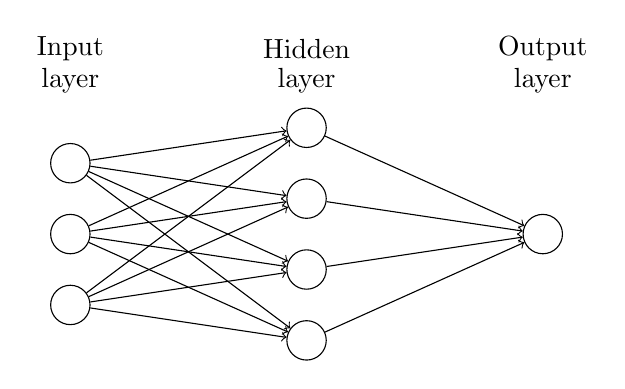
\begin{tikzpicture}
    \node[draw,circle,minimum size=0.5cm] at (3,2.45) (a1) {};
    \node[draw,circle,minimum size=0.5cm] at (3,1.55) (b1) {};
    \node[draw,circle,minimum size=0.5cm] at (3,0.65) (c1) {};

    \node[draw,circle,minimum size=0.5cm] at (6,2.9)  (a2) {};
    \node[draw,circle,minimum size=0.5cm] at (6,2.0)  (b2) {};
    \node[draw,circle,minimum size=0.5cm] at (6,1.1)  (c2) {};
    \node[draw,circle,minimum size=0.5cm] at (6,0.2)  (d2) {};

    \node[draw,circle,minimum size=0.5cm] at (9,1.55) (y)  {};

	\draw[->] (a1) -- (a2);
	\draw[->] (a1) -- (b2);
	\draw[->] (a1) -- (c2);
	\draw[->] (a1) -- (d2);
	\draw[->] (b1) -- (a2);
	\draw[->] (b1) -- (b2);
	\draw[->] (b1) -- (c2);
	\draw[->] (b1) -- (d2);
	\draw[->] (c1) -- (a2);
	\draw[->] (c1) -- (b2);
	\draw[->] (c1) -- (c2);
	\draw[->] (c1) -- (d2);
	\draw[->] (a2) -- (y);
	\draw[->] (b2) -- (y);
	\draw[->] (c2) -- (y);
	\draw[->] (d2) -- (y);

	\node at (3,3.9) {Input};
	\node at (3,3.5) {layer};
	\node at (6,3.9) {Hidden};
	\node at (6,3.5) {layer};
	\node at (9,3.9) {Output};
	\node at (9,3.5) {layer};
	\end{tikzpicture}
	\end{center}
\begin{itemize}
\item Network of artificial neurons, organized in {\color{red} layers}
\item {\color{blue} Fully connected}: each node connects to all nodes in next layer
\item {\color{green} Acyclic}: all edges are left-to-right
\end{itemize}
\end{frame}

\begin{frame}
  \frametitle{Parallel updates}
  \begin{itemize}
	\item Assume that we have a layer of $k$ nodes with shared inputs $x$
	\item For node j, let $w_j$ be its weights and let $s_j=w_j^\top x$
	\item Form the vector of weighted sums $s = (s_1,\ldots,s_k)^\top$
  \begin{align*}
  s &= \left( \begin{array}{ccc} \textrm{-----} & w_1 & \textrm{-----} \\ \textrm{-----} & w_2 & \textrm{-----} \\ & \vdots & \\ \textrm{-----} & w_k & \textrm{-----} \end{array} \right)
  \left( \begin{array}{c} x_0 \\ \vdots \\ x_d \end{array} \right) = W x,
  \end{align*}
	where $W$ is a $k \times (d+1)$ weight matrix
	\item The output vector is given by $o = \varphi(s) = (\varphi(s_1),\ldots,\varphi(s_k))^\top$
  \end{itemize}
\end{frame}

\begin{frame}
  \frametitle{Relationship to supervised learning}
  \begin{itemize}
	\item A feedforward neural network can represent a hypothesis $h(x)$!
	\item Assign inputs $x\in\mathcal{X}$ to neurons in input layer
	\item Propagate values through the network as $o=\varphi(w^\top x)$
	\item Well-defined process since network is acyclic
	\item Predicted output $h(x)\in \mathcal{Y}$: value of neuron(s) in output layer
	\item Usually $\mathcal{Y}=\mathbb{R}$ (regression) or $\mathcal{Y}=[0,1]$ (logistic regression)
  \end{itemize}
\end{frame}

\begin{frame}
\frametitle{Universal approximation theorem}
	\begin{theorem}[Cybenko, 1989; Hornik, 1991]
	A feedforward neural network with a single hidden layer containing a finite number of neurons can approximate any continuous function on a compact subset of $\,\mathbb{R}^n$.
	\end{theorem}
\begin{itemize}
\item Holds for different activation functions
\item Does not imply that the approximation (i.e.~weights) can be {\em learned}
\end{itemize}
\end{frame}

\begin{comment}
\begin{frame}
\frametitle{Example: AND}
  \begin{center}
  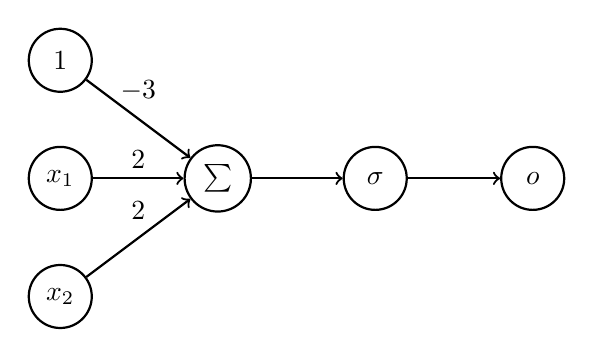
\begin{tikzpicture}
	\node [draw,thick,circle,minimum size=.8cm] at ( 0, 3.5 ) (x0) {$1$};
	\node [draw,thick,circle,minimum size=.8cm] at ( 0, 2 ) (x1) {$x_1$};
	\node [draw,thick,circle,minimum size=.8cm] at ( 0, 0.5 ) (x2) {$x_2$};
	\node [draw,thick,circle,minimum size=.8cm] at ( 2, 2 ) (s) {$\sum$};
	\node [draw,thick,circle,minimum size=.8cm] at ( 4, 2 ) (sig) {$\sigma$};
	\node [draw,thick,circle,minimum size=.8cm] at ( 6, 2 ) (o) {$o$};

	\draw [thick,->] (x0) -- (s) node[above,midway,yshift=.1cm] {$-3$};
	\draw [thick,->] (x1) -- (s) node[above,midway] {$2$};
	\draw [thick,->] (x2) -- (s) node[above,midway,yshift=.1cm] {$2$};
	\draw [thick,->] (s) -- (sig);
	\draw [thick,->] (sig) -- (o);
  \end{tikzpicture}

  \begin{tabular}{|c|c|c|}
	\hline
	$x_1$ & $x_2$ & $x_1\wedge x_2$\\
	\hline
	0 & 0 & 0\\
	0 & 1 & 0\\
	1 & 0 & 0\\
	1 & 1 & 1\\
	\hline
  \end{tabular}
  \end{center}
\end{frame}

\begin{frame}
\frametitle{Example: OR}
  \begin{center}
  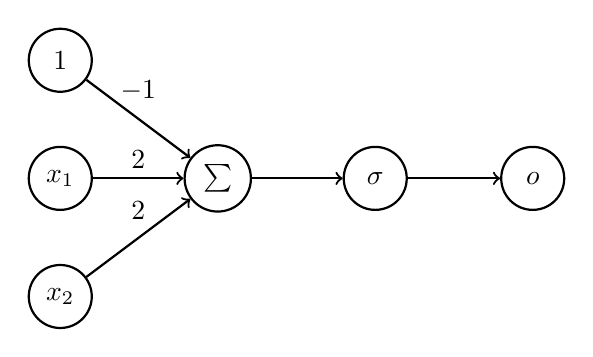
\begin{tikzpicture}
	\node [draw,thick,circle,minimum size=.8cm] at ( 0, 3.5 ) (x0) {$1$};
	\node [draw,thick,circle,minimum size=.8cm] at ( 0, 2 ) (x1) {$x_1$};
	\node [draw,thick,circle,minimum size=.8cm] at ( 0, 0.5 ) (x2) {$x_2$};
	\node [draw,thick,circle,minimum size=.8cm] at ( 2, 2 ) (s) {$\sum$};
	\node [draw,thick,circle,minimum size=.8cm] at ( 4, 2 ) (sig) {$\sigma$};
	\node [draw,thick,circle,minimum size=.8cm] at ( 6, 2 ) (o) {$o$};

	\draw [thick,->] (x0) -- (s) node[above,midway,yshift=.1cm] {$-1$};
	\draw [thick,->] (x1) -- (s) node[above,midway] {$2$};
	\draw [thick,->] (x2) -- (s) node[above,midway,yshift=.1cm] {$2$};
	\draw [thick,->] (s) -- (sig);
	\draw [thick,->] (sig) -- (o);
  \end{tikzpicture}

  \begin{tabular}{|c|c|c|}
	\hline
	$x_1$ & $x_2$ & $x_1\wedge x_2$\\
	\hline
	0 & 0 & 0\\
	0 & 1 & 1\\
	1 & 0 & 1\\
	1 & 1 & 1\\
	\hline
  \end{tabular}
  \end{center}

\end{frame}

\begin{frame}
\frametitle{Example: XOR}
  \begin{center}
  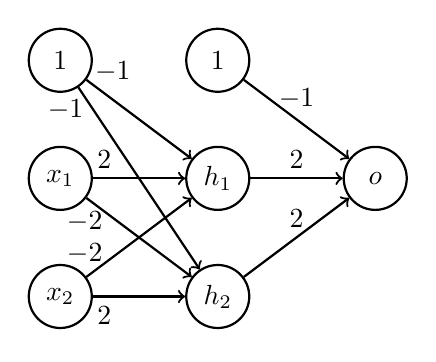
\begin{tikzpicture}
	\node [draw,thick,circle,minimum size=.8cm] at ( 0, 3.5 ) (x0) {$1$};
	\node [draw,thick,circle,minimum size=.8cm] at ( 0, 2 ) (x1) {$x_1$};
	\node [draw,thick,circle,minimum size=.8cm] at ( 0, 0.5 ) (x2) {$x_2$};
	\node [draw,thick,circle,minimum size=.8cm] at ( 2, 3.5 ) (s0) {$1$};
	\node [draw,thick,circle,minimum size=.8cm] at ( 2, 2 ) (s1) {$h_1$};
	\node [draw,thick,circle,minimum size=.8cm] at ( 2, 0.5 ) (s2) {$h_2$};
	\node [draw,thick,circle,minimum size=.8cm] at ( 4, 2 ) (o) {$o$};

	\draw [thick,->] (x0) -- (s1) node[above,near start,yshift=.1cm] {$-1$};
	\draw [thick,->] (x1) -- (s1) node[above,very near start] {$2$};
	\draw [thick,->] (x2) -- (s1) node[left,near start,yshift=.05cm] {$-2$};
	\draw [thick,->] (x0) -- (s2) node[left,very near start] {$-1$};
	\draw [thick,->] (x1) -- (s2) node[left,near start,yshift=-.05cm] {$-2$};
	\draw [thick,->] (x2) -- (s2) node[below,very near start] {$2$};
	\draw [thick,->] (s0) -- (o) node[above,midway] {$-1$};
	\draw [thick,->] (s1) -- (o) node[above,midway] {$2$};
	\draw [thick,->] (s2) -- (o) node[above,midway] {$2$};
  \end{tikzpicture}

  \vspace*{0.6cm}

  \begin{tabular}{|c|c|c|c|c|}
	\hline
	$x_1$ & $x_2$ & $h_1$ & $h_2$ & $x_1\oplus x_2$\\
	\hline
	0 & 0 & 0 & 0 & 0\\
	0 & 1 & 0 & 1 & 1\\
	1 & 0 & 1 & 0 & 1\\
	1 & 1 & 0 & 0 & 0\\
	\hline
  \end{tabular}
  \end{center}

\end{frame}
\end{comment}

\begin{frame}
\frametitle{Backpropagation (various, 1960-1986)}
	\begin{center}
	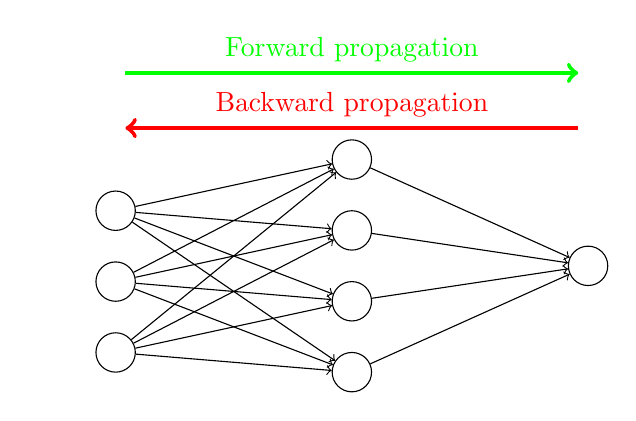
\begin{tikzpicture}
	\node at (2,2.25) (a0) {};
	\node at (2,1.35) (b0) {};
	\node at (2,0.45) (c0) {};

    \node[draw,circle,minimum size=0.5cm] at (3,2.25) (a1) {};
    \node[draw,circle,minimum size=0.5cm] at (3,1.35) (b1) {};
    \node[draw,circle,minimum size=0.5cm] at (3,0.45) (c1) {};

    \node[draw,circle,minimum size=0.5cm] at (6,2.9)  (a2) {};
    \node[draw,circle,minimum size=0.5cm] at (6,2.0)  (b2) {};
    \node[draw,circle,minimum size=0.5cm] at (6,1.1)  (c2) {};
    \node[draw,circle,minimum size=0.5cm] at (6,0.2)  (d2) {};

    \node[draw,circle,minimum size=0.5cm] at (9,1.55) (y)  {};

	\draw[->] (a1) -- (a2);
	\draw[->] (a1) -- (b2);
	\draw[->] (a1) -- (c2);
	\draw[->] (a1) -- (d2);
	\draw[->] (b1) -- (a2);
	\draw[->] (b1) -- (b2);
	\draw[->] (b1) -- (c2);
	\draw[->] (b1) -- (d2);
	\draw[->] (c1) -- (a2);
	\draw[->] (c1) -- (b2);
	\draw[->] (c1) -- (c2);
	\draw[->] (c1) -- (d2);
	\draw[->] (a2) -- (y);
	\draw[->] (b2) -- (y);
	\draw[->] (c2) -- (y);
	\draw[->] (d2) -- (y);

	\node at (3,3.3) (x0) {};
	\node at (9,3.3) (y0) {};
	\node at (3,4.0) (x1) {};
	\node at (9,4.0) (y1) {};

	\draw[->,color=green,ultra thick] (x1) -- (y1) node[midway,above] {\color{green} Forward propagation};
	\draw[->,color=red,ultra thick] (y0) -- (x0) node[midway,above] {\color{red} Backward propagation};
	\end{tikzpicture}
	\end{center}
\begin{itemize}
\item Algorithm for updating the weights in a feedforward network:
\begin{enumerate}
\item Compute gradient of a loss function with respect to weights
\item Update weights from gradient (using {\color{red} gradient descent})
\end{enumerate}
\end{itemize}
\end{frame}

\begin{frame}
\frametitle{Forward propagation}
\begin{itemize}
\item Let $(x_1,\ldots,x_d,y)$ be a training example
\item For each node $j$, compute
\begin{align*}
s_j&=w_j^\top x,\\
o_j&=\varphi(s_j).
\end{align*}
\end{itemize}
\end{frame}

\begin{frame}
\frametitle{Backward propagation}
\begin{itemize}
\item Loss $\ell(h(x),y)=\frac{1}{2}(h(x)-y)^2$ for label $h(x)$ output by network
\item Compute gradient with respect to each weight $w_{ij}$:
\begin{align*}
\frac{\delta \ell(h(x),y)}{\delta w_{ij}}&=\delta_jx_i,\\
\delta_j&=\left\{
\begin{array}{ll}
(o_j-y)\frac{\delta\varphi}{\delta s}(s_j), & j\;\text{is an output node},\\
(\sum_k \delta_kw_{jk})\frac{\delta\varphi}{\delta s}(s_j), & \text{otherwise}.
\end{array}
\right.
\end{align*}
\end{itemize}
\end{frame}

\begin{frame}
\frametitle{Weight update}
\begin{itemize}
\item Stochastic gradient descent in the direction of a minimum error:
\begin{align*}
\Delta w_{ij} &= -\eta\frac{\delta \ell(h(x),y)}{\delta w_{ij}} = -\eta\delta_jx_i.
\end{align*}
\item $\eta$: learning rate
\end{itemize}
\end{frame}

\begin{frame}
\frametitle{Matrix form of backpropagation}
\begin{itemize}
\item Vector of values in layer $k$: $x_k = \varphi_k(W_k x_{k-1})$
\item Vector of deltas in layer $k$:
\[
\delta_k=\left\{
\begin{array}{ll}
(x_k-y) \circ \nabla \varphi_k(W_k x_{k-1}), & k\;\text{is the output layer},\\
W_{k+1}^\top \delta_{k+1} \circ \nabla \varphi_k(W_k x_{k-1}), & \text{otherwise}.
\end{array}
\right.
\]
where $\circ$ is element-wise multiplication (the {\color{red} Hadamard product})
\item Weight updates: $\Delta W_k = -\eta \delta_k x_{k-1}^\top$
\end{itemize}
\end{frame}

\begin{frame}
\frametitle{Limitations of backpropagation}
\begin{itemize}
\item Convergence is slow
\item Needs a lot of data
\item May converge to a local minimum
\item Prone to overfitting (especially when number of nodes is large)
\item Applicable to acyclic networks only
\end{itemize}
\end{frame}

\begin{comment}
\begin{frame}
  \frametitle{Stochastic gradient descent (SGD)}
  \begin{center}
  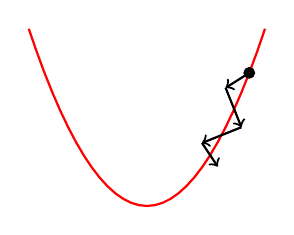
\begin{tikzpicture}
  \draw[thick,red] plot [smooth] (0.5,2.25) -- (0.6,1.96) -- (0.7,1.69) -- (0.8,1.44) -- (0.9,1.21) -- (1,1) -- (1.1,0.81) -- (1.2,0.64) -- (1.3,0.49) -- (1.4,0.36) -- (1.5,0.25) -- (1.6,0.16) -- (1.7,0.09) -- (1.8,0.04) -- (1.9,0.01) -- (2,0) -- (2.1,0.01) -- (2.2,0.04) -- (2.3,0.09) -- (2.4,0.16) -- (2.5,0.25) -- (2.6,0.36) -- (2.7,0.49) -- (2.8,0.64) -- (2.9,0.81) -- (3,1) -- (3.1,1.21) -- (3.2,1.44) -- (3.3,1.69) -- (3.4,1.96) -- (3.5,2.25);
  \draw[thick,fill=black] (3.3,1.69) circle (0.06cm);
  \draw[thick,->] (3.3,1.69) -- (3,1.5);
  \draw[thick,->] (3,1.5) -- (3.2,1);
  \draw[thick,->] (3.2,1) -- (2.7,0.8);
  \draw[thick,->] (2.7,0.8) -- (2.9,0.5);
  \end{tikzpicture}
  \end{center}
  \begin{itemize}
	\item If the training set $S$ is large, computing $\nabla_wL_S(w)$ is expensive
	\item Idea: compute {\color{blue} partial gradient} on subset of data points
	\item Each partial gradient does not coincide with the full gradient
	\item In {\color{green} expectation}, partial gradients descend towards minimum
  \end{itemize}
\end{frame}

\begin{frame}
  \frametitle{Partial gradient}
  \begin{itemize}
	\item Given weight vector $w$, several ways to compute partial gradient:
	\begin{enumerate}
	\item Compute gradient of loss function $\ell(h(x),y)$ on {\color{red} data point $(x,y)$}
	\item Compute partial gradient on {\color{blue} mini-batch} $S'\subset S$, $|S'| \ll |S|$
	\end{enumerate}
  \end{itemize}
\end{frame}

\begin{frame}
  \frametitle{Subgradients}
  \begin{center}
  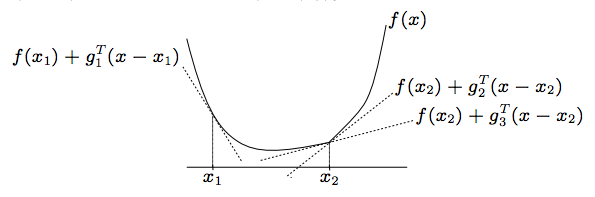
\includegraphics[height=3cm]{images/subgradient.png}
  \end{center}
  \begin{itemize}
	\item Some functions (such as ReLU) are not differentiable everywhere
	\item It may still be possible to compute {\color{red} subgradients}
  \end{itemize}
\end{frame}
\end{comment}

\begin{frame}
  \frametitle{Multiclass classification}
  \begin{center}
  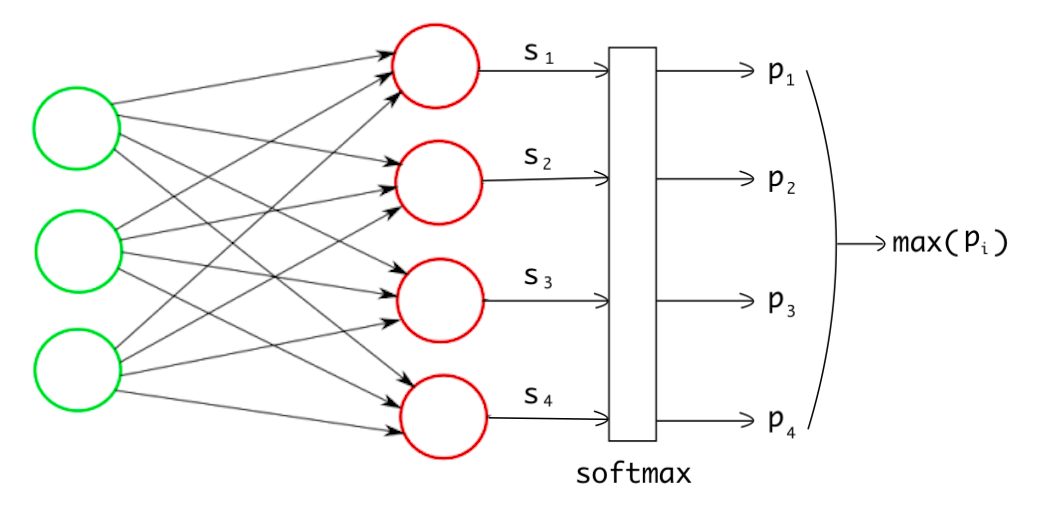
\includegraphics[height=4cm]{images/softmax.png}
  \end{center}
  \begin{itemize}
	\item To assign probabilities to multiple classes, must {\color{red} normalize} output
	\item {\color{blue} Softmax layer}: 
	\[\mathbb{P}(y=k|x) = \frac {e^{w_k^\top x}} {\sum_j e^{w_j^\top x}}\]
  \end{itemize}
\end{frame}

\begin{frame}
  \frametitle{Effect of softmax normalization}
  \begin{center}
  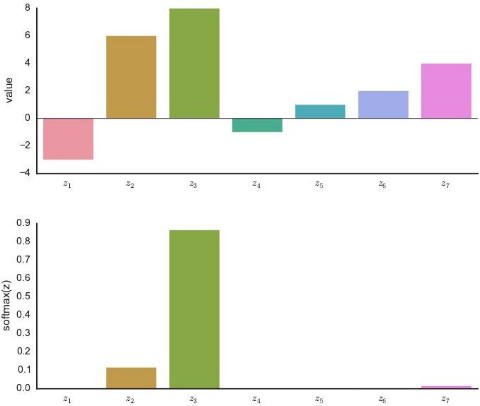
\includegraphics[height=6cm]{images/norm.png}
  \end{center}
\end{frame}

\section{Deep learning}

\begin{frame}
\frametitle{Deep learning}
	\begin{center}
	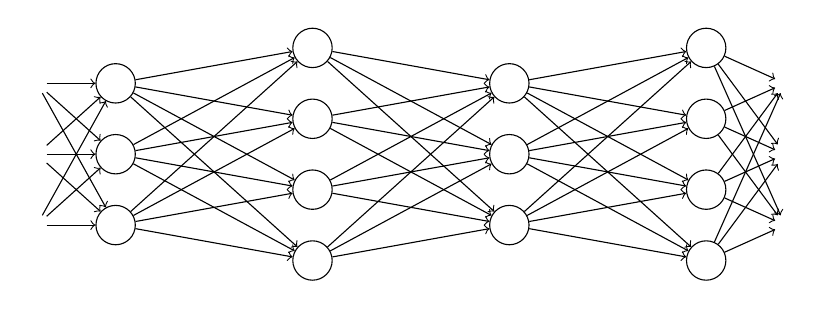
\begin{tikzpicture}
	\node at (0,2.45) (a0) {};
	\node at (0,1.55) (b0) {};
	\node at (0,0.65) (c0) {};

    \node[draw,circle,minimum size=0.5cm] at (1,2.45) (a1) {};
    \node[draw,circle,minimum size=0.5cm] at (1,1.55) (b1) {};
    \node[draw,circle,minimum size=0.5cm] at (1,0.65) (c1) {};

    \node[draw,circle,minimum size=0.5cm] at (3.5,2.9) (a2) {};
    \node[draw,circle,minimum size=0.5cm] at (3.5,2.0) (b2) {};
    \node[draw,circle,minimum size=0.5cm] at (3.5,1.1) (c2) {};
    \node[draw,circle,minimum size=0.5cm] at (3.5,0.2) (d2) {};

    \node[draw,circle,minimum size=0.5cm] at (6,2.45) (a3) {};
    \node[draw,circle,minimum size=0.5cm] at (6,1.55) (b3) {};
    \node[draw,circle,minimum size=0.5cm] at (6,0.65) (c3) {};

    \node[draw,circle,minimum size=0.5cm] at (8.5,2.9) (a4) {};
    \node[draw,circle,minimum size=0.5cm] at (8.5,2.0) (b4) {};
    \node[draw,circle,minimum size=0.5cm] at (8.5,1.1) (c4) {};
    \node[draw,circle,minimum size=0.5cm] at (8.5,0.2) (d4) {};

	\node at (9.5,2.45) (a5) {};
	\node at (9.5,1.55) (b5) {};
	\node at (9.5,0.65) (c5) {};

	\draw[->] (a0) -- (a1);
	\draw[->] (a0) -- (b1);
	\draw[->] (a0) -- (c1);
	\draw[->] (b0) -- (a1);
	\draw[->] (b0) -- (b1);
	\draw[->] (b0) -- (c1);
	\draw[->] (c0) -- (a1);
	\draw[->] (c0) -- (b1);
	\draw[->] (c0) -- (c1);
	\draw[->] (a1) -- (a2);
	\draw[->] (a1) -- (b2);
	\draw[->] (a1) -- (c2);
	\draw[->] (a1) -- (d2);
	\draw[->] (b1) -- (a2);
	\draw[->] (b1) -- (b2);
	\draw[->] (b1) -- (c2);
	\draw[->] (b1) -- (d2);
	\draw[->] (c1) -- (a2);
	\draw[->] (c1) -- (b2);
	\draw[->] (c1) -- (c2);
	\draw[->] (c1) -- (d2);
	\draw[->] (a2) -- (a3);
	\draw[->] (a2) -- (b3);
	\draw[->] (a2) -- (c3);
	\draw[->] (b2) -- (a3);
	\draw[->] (b2) -- (b3);
	\draw[->] (b2) -- (c3);
	\draw[->] (c2) -- (a3);
	\draw[->] (c2) -- (b3);
	\draw[->] (c2) -- (c3);
	\draw[->] (d2) -- (a3);
	\draw[->] (d2) -- (b3);
	\draw[->] (d2) -- (c3);
	\draw[->] (a3) -- (a4);
	\draw[->] (a3) -- (b4);
	\draw[->] (a3) -- (c4);
	\draw[->] (a3) -- (d4);
	\draw[->] (b3) -- (a4);
	\draw[->] (b3) -- (b4);
	\draw[->] (b3) -- (c4);
	\draw[->] (b3) -- (d4);
	\draw[->] (c3) -- (a4);
	\draw[->] (c3) -- (b4);
	\draw[->] (c3) -- (c4);
	\draw[->] (c3) -- (d4);
	\draw[->] (a4) -- (a5);
	\draw[->] (a4) -- (b5);
	\draw[->] (a4) -- (c5);
	\draw[->] (b4) -- (a5);
	\draw[->] (b4) -- (b5);
	\draw[->] (b4) -- (c5);
	\draw[->] (c4) -- (a5);
	\draw[->] (c4) -- (b5);
	\draw[->] (c4) -- (c5);
	\draw[->] (d4) -- (a5);
	\draw[->] (d4) -- (b5);
	\draw[->] (d4) -- (c5);
	\end{tikzpicture}
	\end{center}
\begin{itemize}
\item Use cascades of many hidden layers of processing units ($>2$)
\item Combinations of different types of layers
\end{itemize}
\end{frame}

\begin{frame}
\frametitle{Development set}
  \begin{center}
  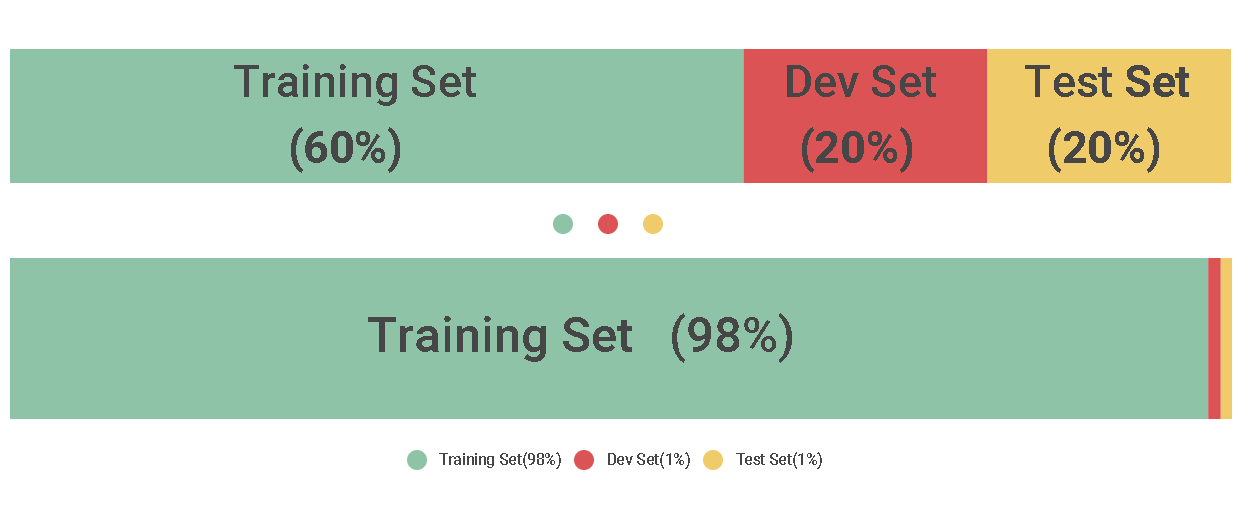
\includegraphics[height=4cm]{images/devset.png}
  \end{center}
\end{frame}

\begin{frame}
\frametitle{Learning curves}
  \begin{center}
  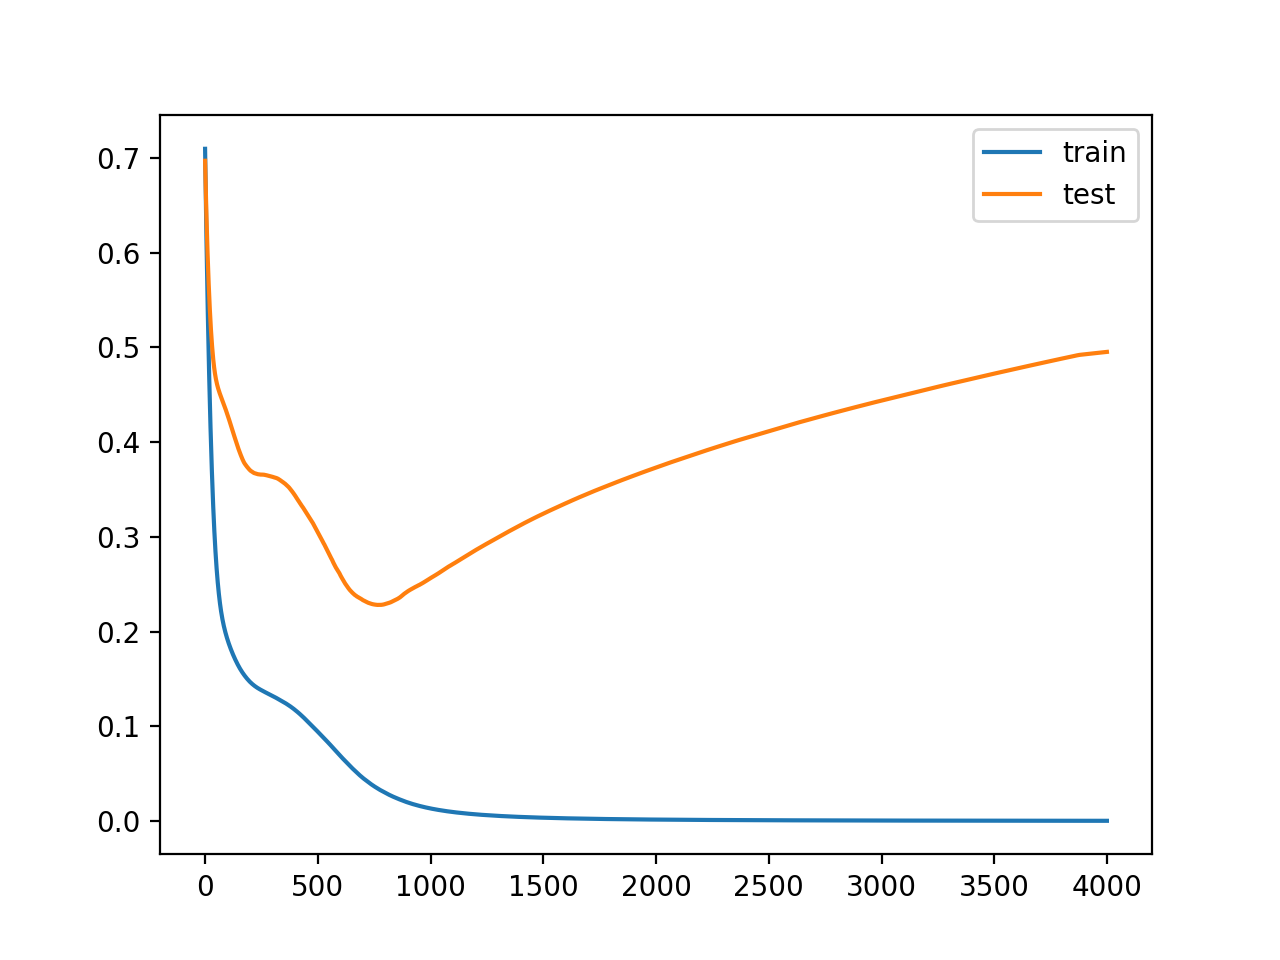
\includegraphics[height=5cm]{images/validation.png}
  \end{center}
  \begin{itemize}
	\item Compute validation error after each epoch, save snapshots
	\item Monitor validation error as a function of the number of epochs
  \end{itemize}
\end{frame}

\begin{frame}
\frametitle{Optimizers}
  \begin{center}
  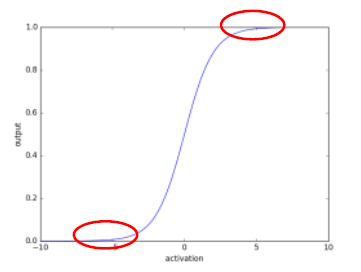
\includegraphics[height=4cm]{images/optimize.png}
  \end{center}
  \begin{itemize}
	\item In the flat part of the sigmoid, gradient is close to 0
	\item {\color{red} Optimizers} adapt the learning rate to account for gradient slope
  \end{itemize}
\end{frame}

\begin{frame}
\frametitle{Overfitting}
\begin{itemize}
\item Effect of overfitting increases as networks become larger
\item Deep learning usually applies {\color{red} regularization}:
\begin{itemize}
\item Sparsity ($L_1$-regularization)
\item Weight decay ($L_2$-regularization)
\item {\color{blue} Dropout regularization} (specific to neural networks)
\end{itemize}
\end{itemize}
\end{frame}

\begin{frame}
\frametitle{Dropout regularization}
	\begin{center}
	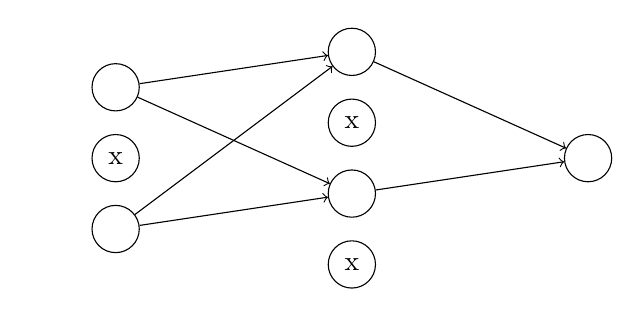
\begin{tikzpicture}
	\node at (2,2.45) (a0) {};
	\node at (2,1.55) (b0) {};
	\node at (2,0.65) (c0) {};

    \node[draw,circle,minimum size=0.6cm] at (3,2.45) (a1) {};
    \node[draw,circle,minimum size=0.6cm] at (3,1.55) (b1) {x};
    \node[draw,circle,minimum size=0.6cm] at (3,0.65) (c1) {};

    \node[draw,circle,minimum size=0.6cm] at (6,2.9) (a2) {};
    \node[draw,circle,minimum size=0.6cm] at (6,2.0) (b2) {x};
    \node[draw,circle,minimum size=0.6cm] at (6,1.1) (c2) {};
    \node[draw,circle,minimum size=0.6cm] at (6,0.2) (d2) {x};

    \node[draw,circle,minimum size=0.6cm] at (9,1.55) (y)  {};

	\draw[->] (a1) -- (a2);
	\draw[->] (a1) -- (c2);
	\draw[->] (c1) -- (a2);
	\draw[->] (c1) -- (c2);
	\draw[->] (a2) -- (y);
	\draw[->] (c2) -- (y);
	\end{tikzpicture}
	\end{center}
\begin{itemize}
\item Averaging over multiple networks is very slow
\item Idea: randomly drop nodes from network during training
\end{itemize}
\end{frame}

\begin{frame}
\frametitle{Hyperparameters}
  All parameters that describe the learning process:

  \vspace*{0.2cm}

  \begin{itemize}
	\item Activation function $\varphi$
	\item Number of hidden layers
	\item Number of nodes in each hidden layer
	\item Weight initialization
	\item Learning rate $\eta$
	\item Number of training epochs $T$
	\item Size of minibatches for backpropagation
	\item Algorithm used for SGD
	\item Regularization scheme
	\item etc. etc.
  \end{itemize}
\end{frame}

\begin{frame}
\frametitle{Hyperparameter engineering}
  \begin{center}
  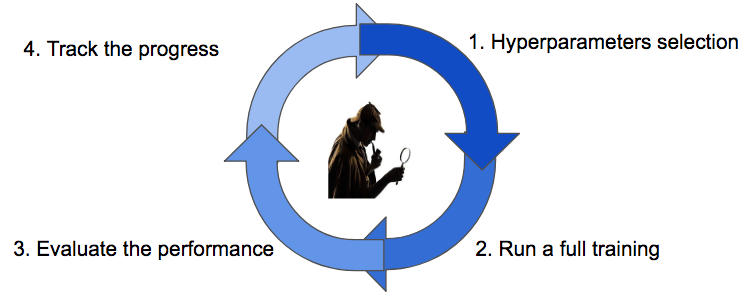
\includegraphics[height=4.5cm]{images/hyperpars.png}
  \end{center}
\end{frame}

\begin{frame}
\frametitle{Advantages of deep learning}
\begin{itemize}
\item Flexible design
\item End-to-end, automatic feature discovery
\item High-level features learned from low-level features
\item State-of-the-art performance in many applications
\end{itemize}
\end{frame}

\begin{frame}
\frametitle{Criticism}
\begin{itemize}
\item Lots of engineering!
\item Lack of transparency
\item Lack of theoretical foundations
\item Same accuracy achievable using fewer nodes
\end{itemize}
\end{frame}

\section{Convolutional neural networks}

\begin{frame}
\frametitle{Image data}
\begin{center}
\begin{tabular}{ccc}
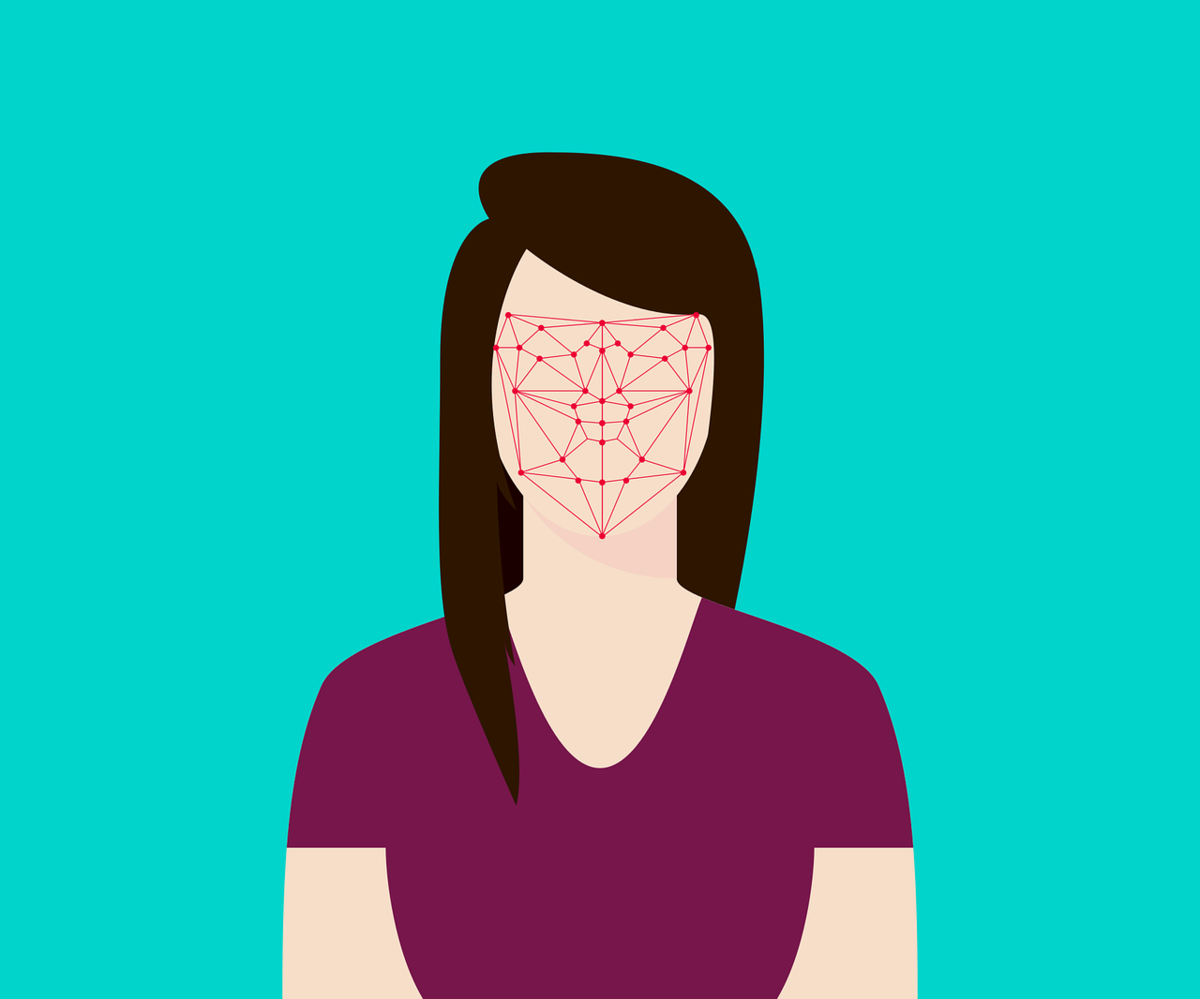
\includegraphics[height=2.5cm]{images/Face_Recognition.png}
& 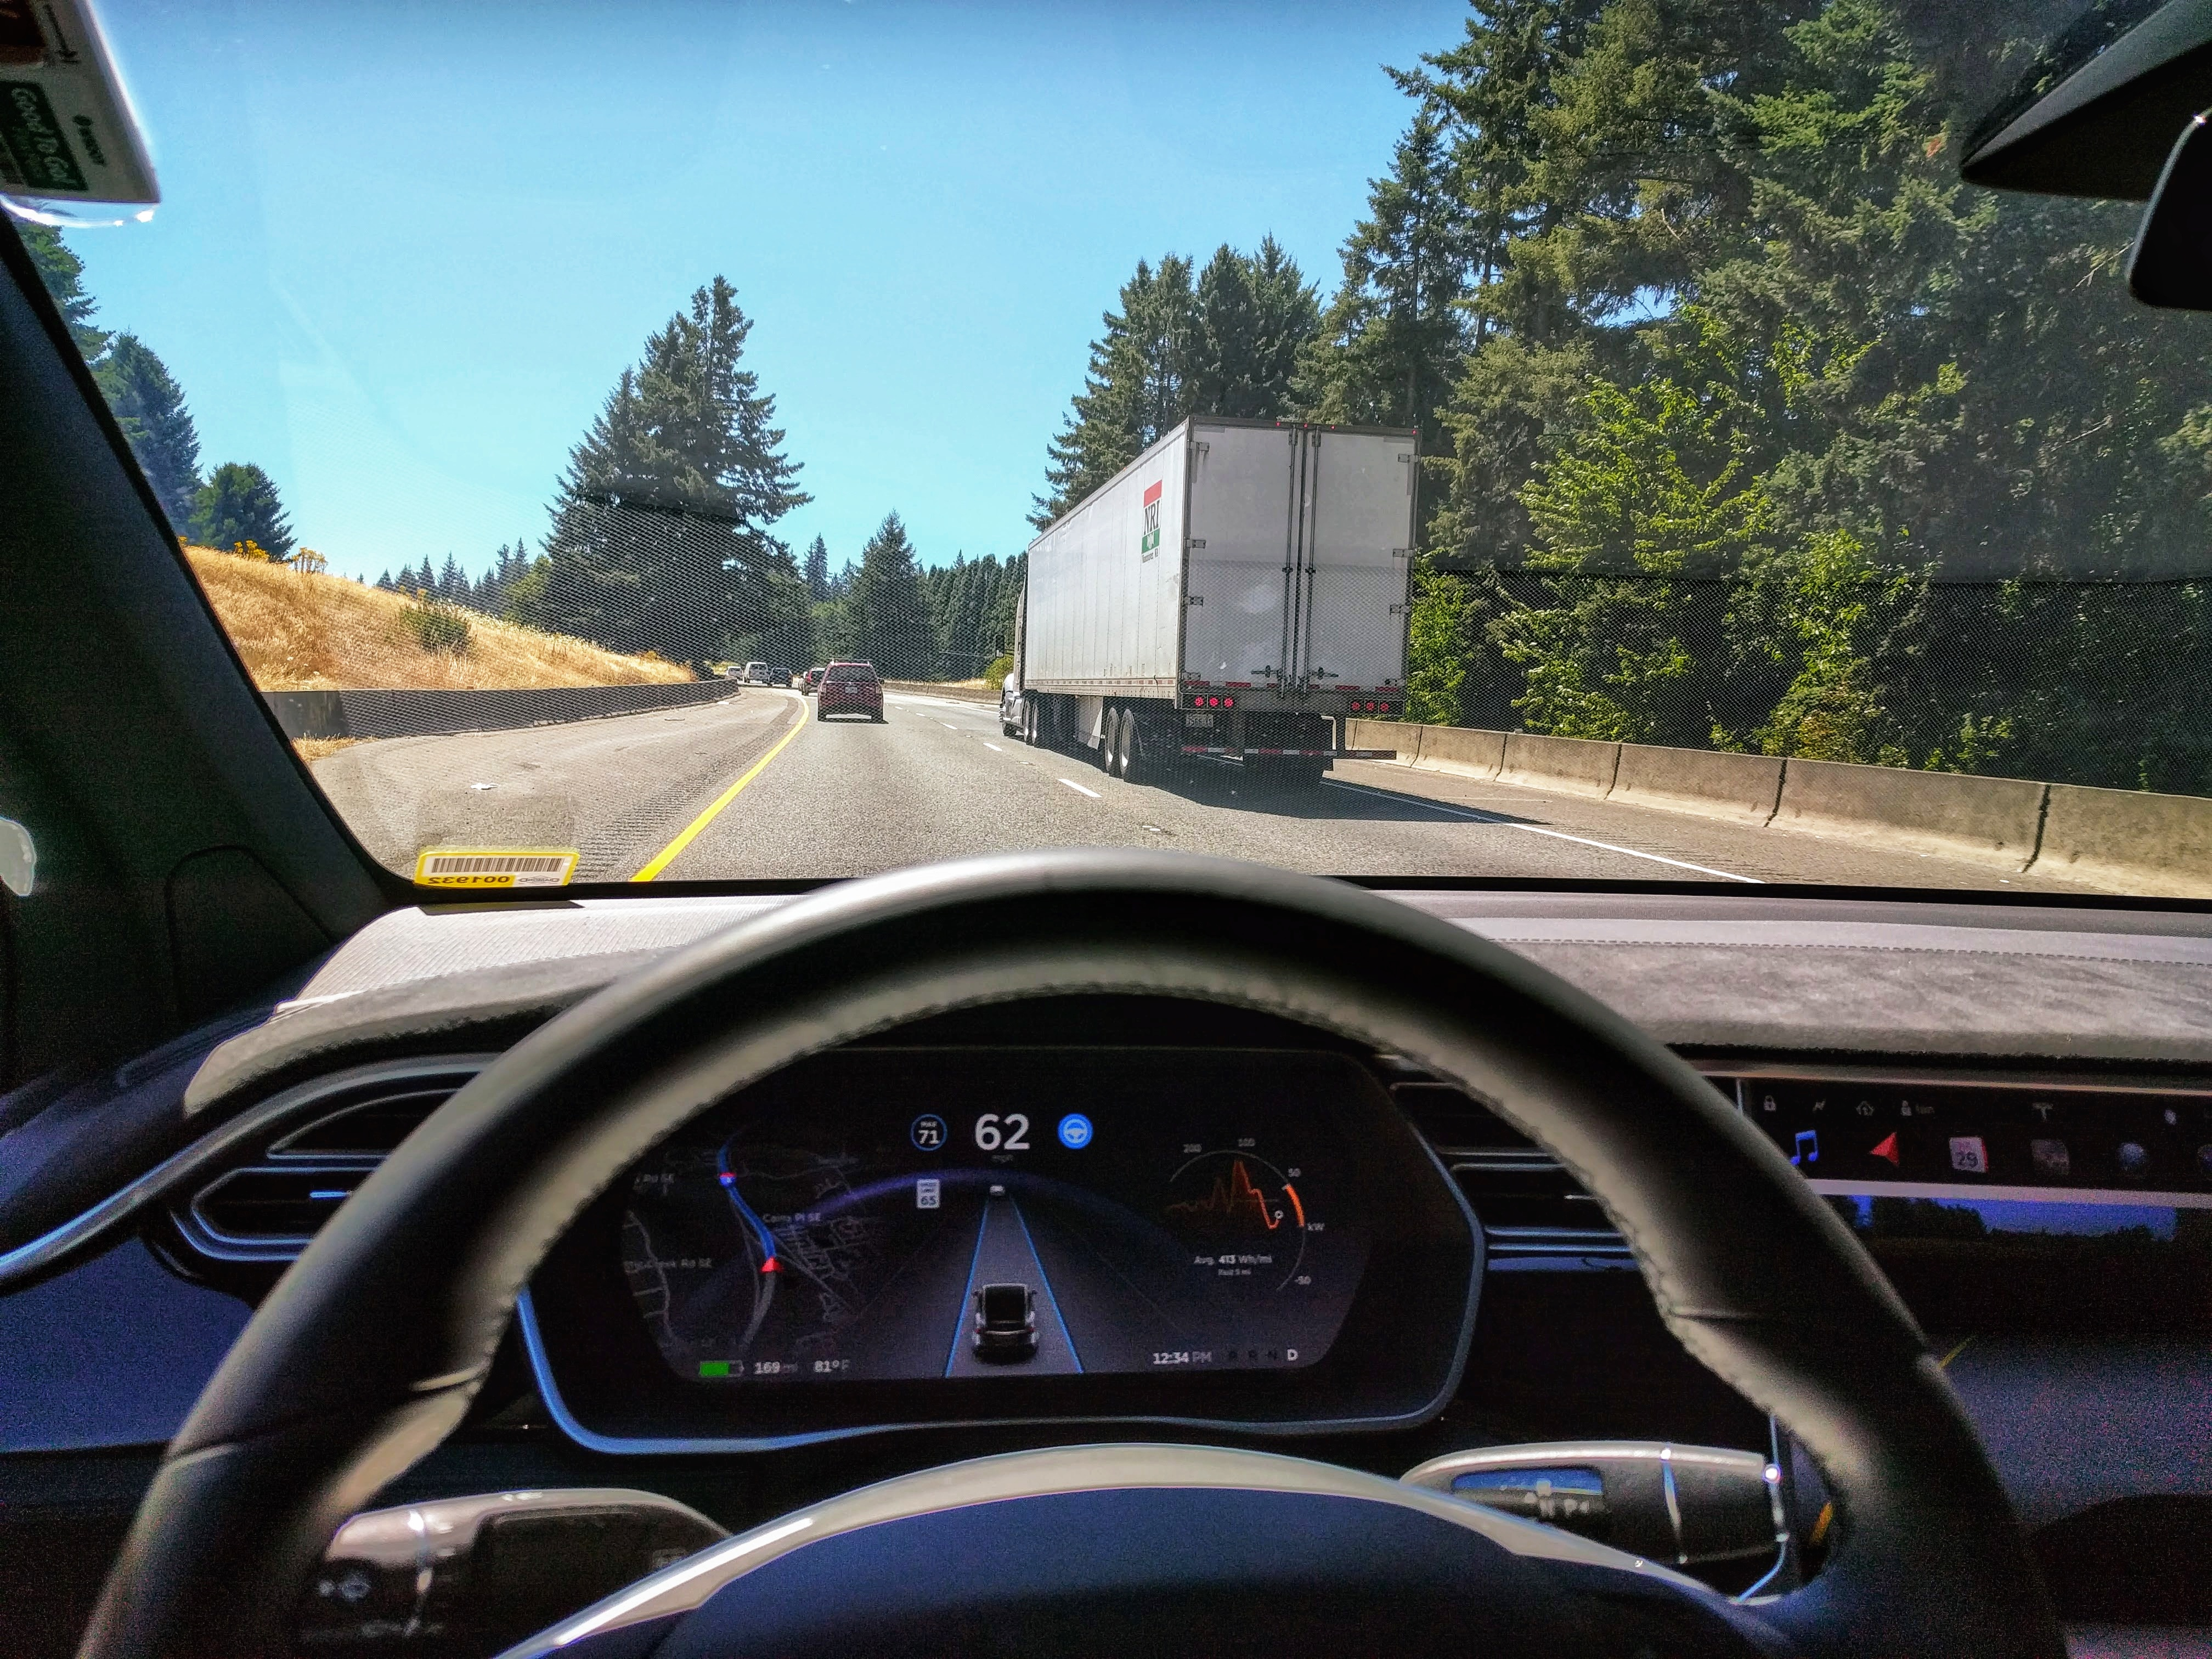
\includegraphics[height=2.5cm]{images/Tesla.jpg}
& 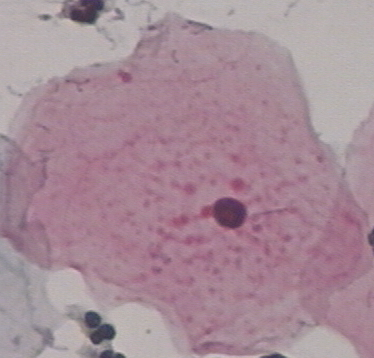
\includegraphics[height=2.5cm]{images/img1.png}
\end{tabular}
\end{center}
\begin{itemize}
\item Many applications are based on visual input
\item How do we adapt neural networks to image data?
\end{itemize}
\end{frame}

\begin{frame}
\frametitle{Input dimensionality}
\begin{center}
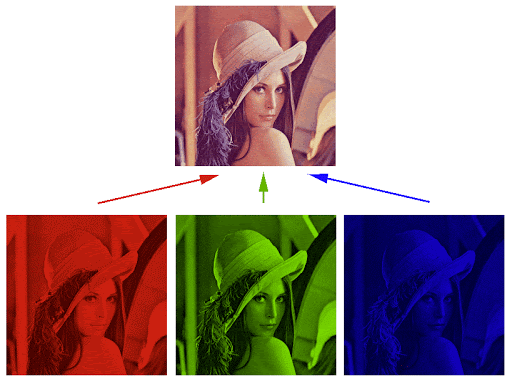
\includegraphics[height=4.5cm]{images/rgb.png}
\end{center}
\begin{itemize}
\item A common image resolution is $1{,}024 \times 768 = 786{,}432$ pixels
\item Each pixel is defined by three colors ({\color{red}R}{\color{green}G}{\color{blue}B})
\item $1{,}000$ nodes in first hidden layer $\Rightarrow$ {\color{red} $\geq 2{,}000{,}000{,}000$ weights!}
\end{itemize}
\end{frame}

\begin{frame}
\frametitle{Visual cortex}
\centerline{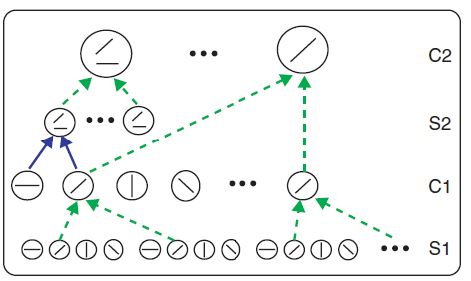
\includegraphics[height=4cm]{images/cortex.png}}
\begin{itemize}
\item Cells in visual cortex track features of increasing complexity
\item Neurons act as {\color{red} local filters} over the input space
\end{itemize}
\end{frame}

\begin{frame}
\frametitle{From low to high level features}
\centerline{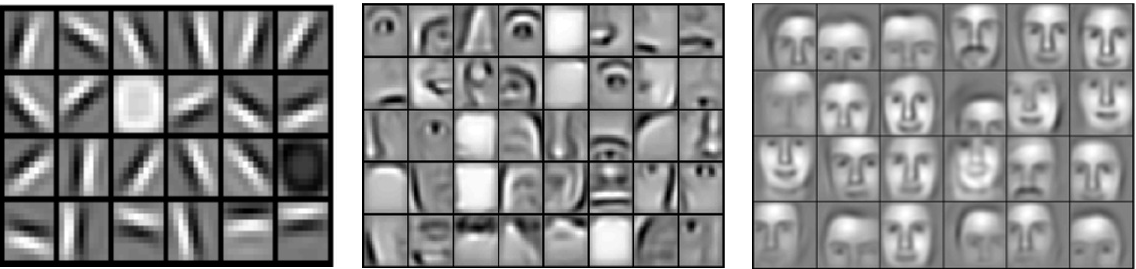
\includegraphics[height=2.5cm]{images/features.png}}

\begin{center}
\begin{tabular}{ccc}
Low-level \hspace*{1.1cm} & Small structure & \hspace*{1.4cm} High-level
\end{tabular}
\end{center}
\end{frame}

\begin{frame}
\frametitle{Edge detection}
\centerline{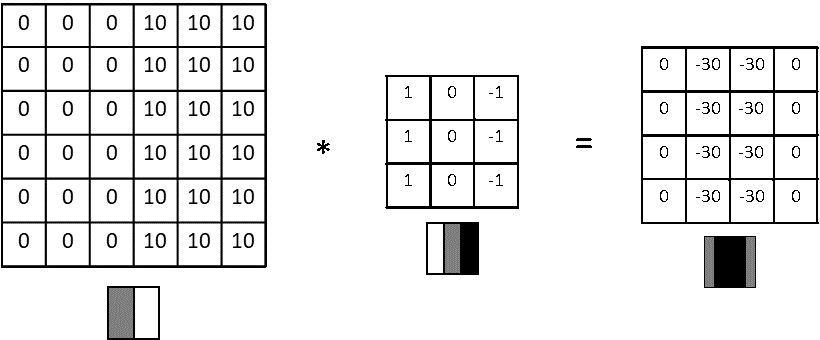
\includegraphics[height=4.5cm]{images/edgedet.png}}
\begin{itemize}
\item We can use small filters to detect low-level features
\item These filters are {\color{red} repeated} over the entire image
\end{itemize}
\end{frame}

\begin{frame}
\frametitle{Convolutional layer}
\centerline{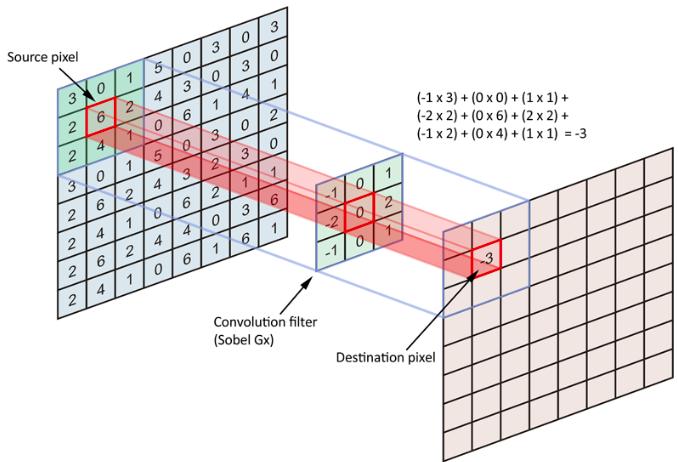
\includegraphics[height=7cm]{images/convlayer.png}}
\end{frame}

\begin{frame}
\frametitle{Generalized edge detection}
\begin{center}
  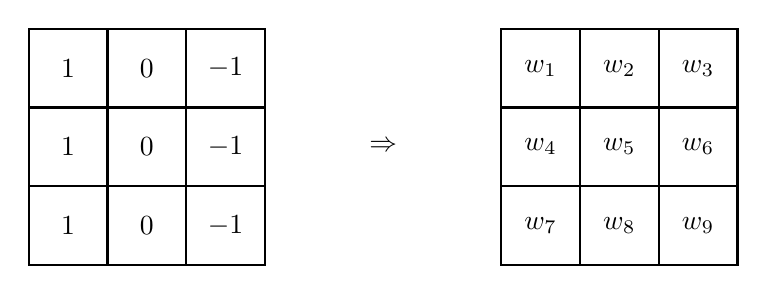
\begin{tikzpicture}
	\node [draw,thick,minimum size=1cm] at ( 1,1 ) {$1$};
	\node [draw,thick,minimum size=1cm] at ( 2,1 ) {$0$};
	\node [draw,thick,minimum size=1cm] at ( 3,1 ) {$-1$};
	\node [draw,thick,minimum size=1cm] at ( 1,2 ) {$1$};
	\node [draw,thick,minimum size=1cm] at ( 2,2 ) {$0$};
	\node [draw,thick,minimum size=1cm] at ( 3,2 ) {$-1$};
	\node [draw,thick,minimum size=1cm] at ( 1,3 ) {$1$};
	\node [draw,thick,minimum size=1cm] at ( 2,3 ) {$0$};
	\node [draw,thick,minimum size=1cm] at ( 3,3 ) {$-1$};

	\node at (5,2) {$\Rightarrow$};

	\node [draw,thick,minimum size=1cm] at ( 7,1 ) {$w_7$};
	\node [draw,thick,minimum size=1cm] at ( 8,1 ) {$w_8$};
	\node [draw,thick,minimum size=1cm] at ( 9,1 ) {$w_9$};
	\node [draw,thick,minimum size=1cm] at ( 7,2 ) {$w_4$};
	\node [draw,thick,minimum size=1cm] at ( 8,2 ) {$w_5$};
	\node [draw,thick,minimum size=1cm] at ( 9,2 ) {$w_6$};
	\node [draw,thick,minimum size=1cm] at ( 7,3 ) {$w_1$};
	\node [draw,thick,minimum size=1cm] at ( 8,3 ) {$w_2$};
	\node [draw,thick,minimum size=1cm] at ( 9,3 ) {$w_3$};
  \end{tikzpicture}
\end{center}
\begin{itemize}
\item Use backpropagation to {\color{red} automatically} learn filters
\item Still repeat the same small filters over the entire image
\end{itemize}
\end{frame}

\begin{frame}
\frametitle{Shrinking}
\begin{center}
  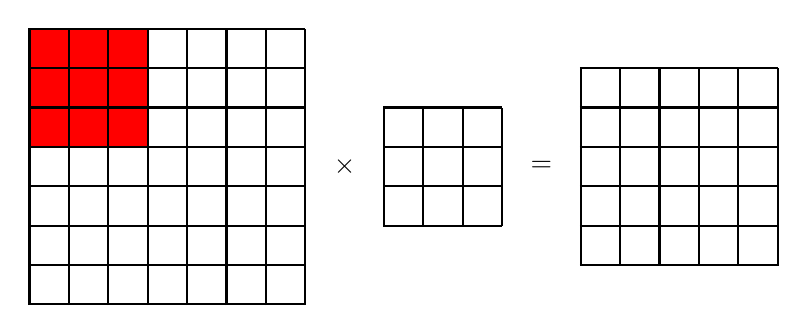
\begin{tikzpicture}
	\draw[black,thick,fill=red] (1,3) rectangle (2.5,4.5);
	\draw[step=0.5,black,thick] (0.99,0.99) grid (4.5,4.5);
	\node at (5, 2.75) {$\times$};
	\draw[step=0.5,black,thick] (5.49,1.99) grid (7,3.5);
	\node at (7.5, 2.75) {$=$};
	\draw[step=0.5,black,thick] (7.99,1.49) grid (10.5,4);
  \end{tikzpicture}
\end{center}
\begin{itemize}
\item Applying a filter causes the image size to {\color{red} shrink}
\end{itemize}
\end{frame}

\begin{frame}
\frametitle{Padding}
\begin{center}
  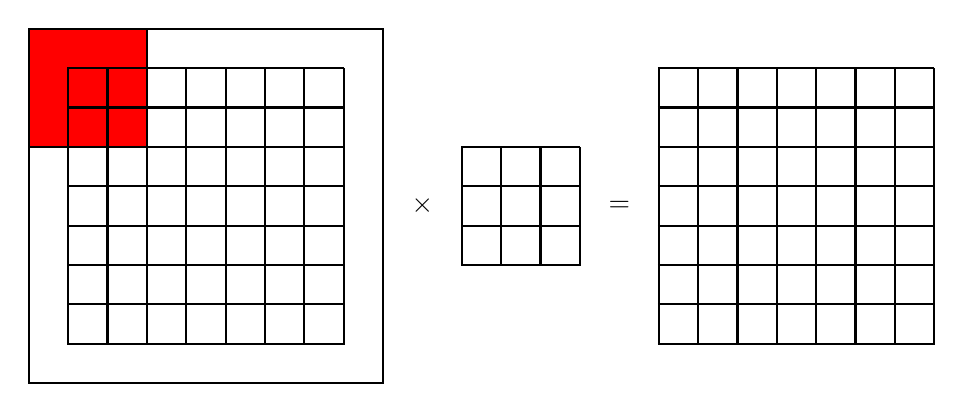
\begin{tikzpicture}
	\draw[black,thick,fill=red] (0.5,3.5) rectangle (2,5);
	\draw[black,thick] (0.5,0.5) rectangle (5,5);
	\draw[step=0.5,black,thick] (0.99,0.99) grid (4.5,4.5);
	\node at (5.5, 2.75) {$\times$};
	\draw[step=0.5,black,thick] (5.99,1.99) grid (7.5,3.5);
	\node at (8, 2.75) {$=$};
	\draw[step=0.5,black,thick] (8.49,0.99) grid (12,4.5);
  \end{tikzpicture}
\end{center}
\begin{itemize}
\item {\color{red} Padding}: add dummy pixels in all directions (usually with value $0$)
\end{itemize}
\end{frame}

\begin{frame}
\frametitle{Stride}
\begin{center}
  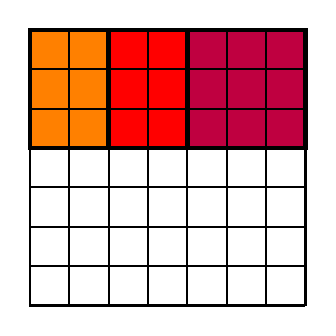
\begin{tikzpicture}
	\draw[black,ultra thick,fill=orange] (1,3) rectangle (2.5,4.5);
	\draw[black,ultra thick,fill=red] (2,3) rectangle (3.5,4.5);
	\draw[black,ultra thick,fill=purple] (3,3) rectangle (4.5,4.5);
	\draw[step=0.5,black,thick] (0.99,0.99) grid (4.5,4.5);
  \end{tikzpicture}
\end{center}
\begin{itemize}
\item {\color{red} Stride}: how many steps we move the filter in each iteration
\end{itemize}
\end{frame}

\begin{frame}
\frametitle{Convolution over volumes}
\centerline{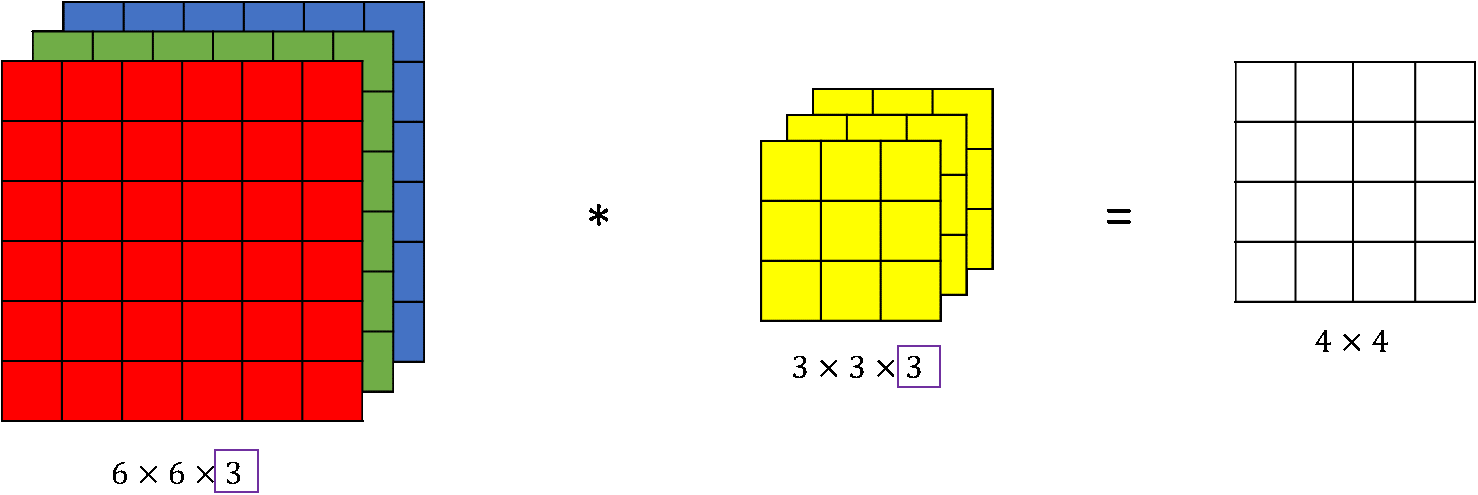
\includegraphics[height=3.5cm]{images/volumes.png}}
\begin{itemize}
\item Filters can be three-dimensional!
\item Can capture full color profile of local neighborhoods
\end{itemize}
\end{frame}

\begin{frame}
\frametitle{Multiple filters}
\centerline{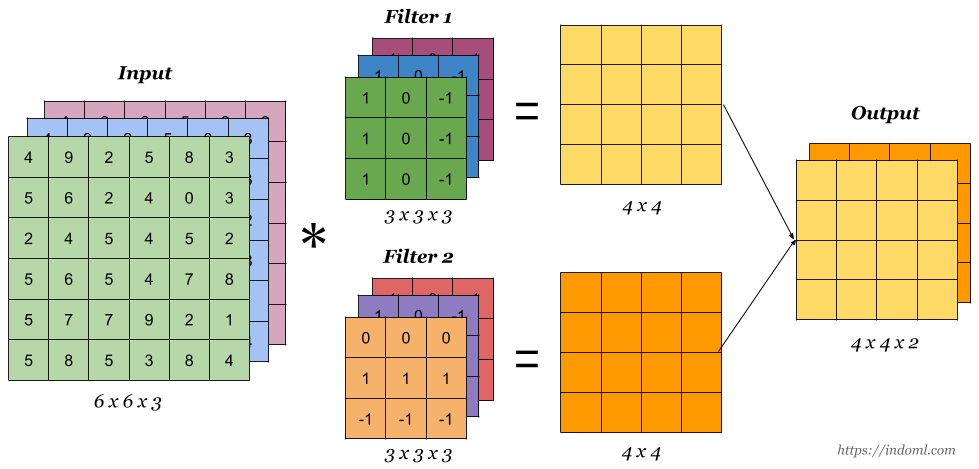
\includegraphics[height=5.5cm]{images/multiple.png}}
\begin{itemize}
\item Typically we apply {\color{red} many} filters to the same image
\end{itemize}
\end{frame}

\begin{frame}
\frametitle{Convolutional neural network (CNN)}
\centerline{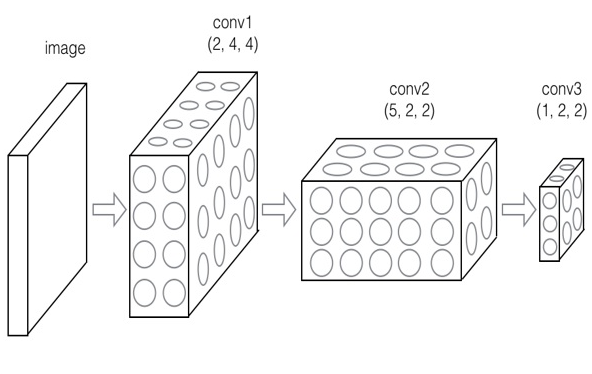
\includegraphics[height=4cm]{images/conv.png}}
\begin{itemize}
\item Multiple filters arranged in several layers
\item Approximates the mechanism of the visual cortex 
\end{itemize}
\end{frame}

\begin{frame}
\frametitle{Convolutional layer}
	\begin{center}
	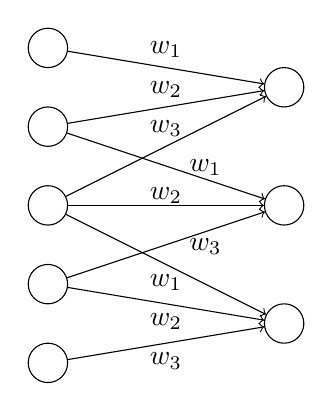
\begin{tikzpicture}
    \node[draw,circle,minimum size=0.5cm] at (3,4.15) (a1) {};
    \node[draw,circle,minimum size=0.5cm] at (3,3.15) (b1) {};
    \node[draw,circle,minimum size=0.5cm] at (3,2.15) (c1) {};
    \node[draw,circle,minimum size=0.5cm] at (3,1.15) (d1) {};
    \node[draw,circle,minimum size=0.5cm] at (3,0.15) (e1) {};

    \node[draw,circle,minimum size=0.5cm] at (6,3.65) (a2) {};
    \node[draw,circle,minimum size=0.5cm] at (6,2.15) (b2) {};
    \node[draw,circle,minimum size=0.5cm] at (6,0.65) (c2) {};
	
    \draw[->] (a1) -- (a2) node[midway,above] {$w_1$};
    \draw[->] (b1) -- (a2) node[midway,above] {$w_2$};
    \draw[->] (c1) -- (a2) node[midway,above] {$w_3$};
    \draw[->] (b1) -- (b2) node[midway,above,xshift=.5cm,yshift=-.25cm] {$w_1$};
    \draw[->] (c1) -- (b2) node[midway,above,yshift=-.1cm] {$w_2$};
    \draw[->] (d1) -- (b2) node[midway,below,xshift=.5cm,yshift=.2cm] {$w_3$};
    \draw[->] (c1) -- (c2) node[midway,below] {$w_1$};
    \draw[->] (d1) -- (c2) node[midway,below] {$w_2$};
    \draw[->] (e1) -- (c2) node[midway,below] {$w_3$};
	\end{tikzpicture}
	\end{center}
\begin{itemize}
\item {\em Not} fully connected
\item Each pattern replicated over the entire input
\item Weights are shared!
\end{itemize}
\end{frame}

\begin{frame}
\frametitle{Input dimensionality}
\begin{center}
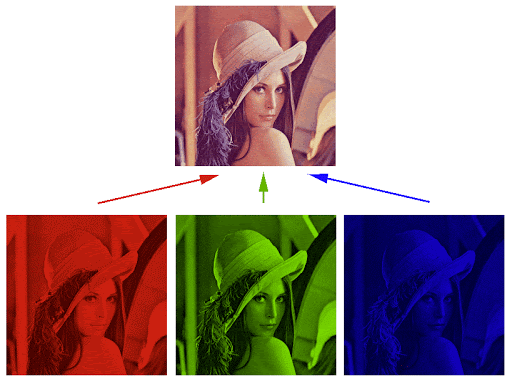
\includegraphics[height=4.5cm]{images/rgb.png}
\end{center}
\begin{itemize}
\item $k$ filters of size $n\times n \times 3$ $\Rightarrow$ {\color{red} $3k\cdot n^2$ weights}
\item Independent of the number of pixels!
\item $100$ filters of size $100\times 100 \times 3$ $\Rightarrow$ {\color{blue} $3{,}000{,}000 \ll 2{,}000{,}000{,}000$}
\end{itemize}
\end{frame}

\begin{frame}
\frametitle{Matrix operations}
\begin{center}
\raisebox{-0.4\height}{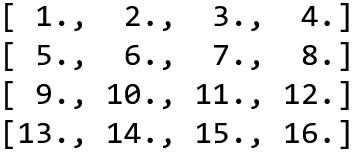
\includegraphics[height=3cm]{images/WA.png}} {\LARGE *} \raisebox{-0.25\height}{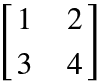
\includegraphics[height=1.5cm]{images/Q.png}}
\end{center}
\end{frame}

\begin{frame}
\frametitle{Matrix operations}
\begin{center}
\raisebox{-0.25\height}{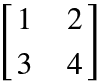
\includegraphics[height=1.2cm]{images/Q.png}} \hspace*{.2cm} \raisebox{-0.4\height}{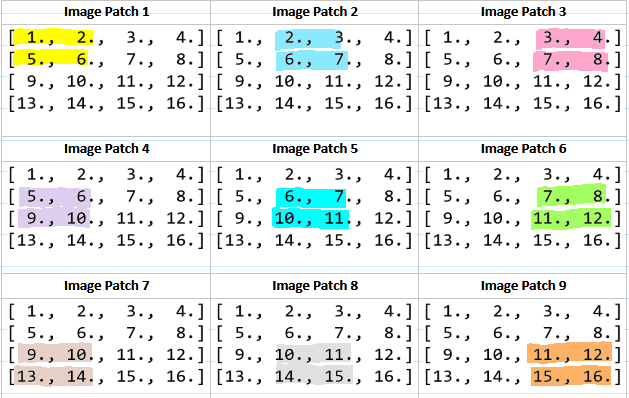
\includegraphics[height=4.5cm]{images/convo.png}}\\
$\Downarrow$\\
\raisebox{-0.05\height}{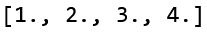
\includegraphics[height=0.4cm]{images/Qflat.png}}
\raisebox{-0.35\height}{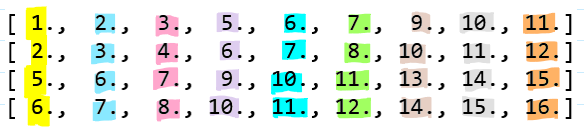
\includegraphics[height=1.5cm]{images/flatten.png}}
\end{center}
\end{frame}

\begin{frame}
\frametitle{Matrix operations}
\begin{center}
\raisebox{-0.05\height}{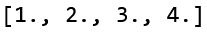
\includegraphics[height=0.4cm]{images/Qflat.png}}
\raisebox{-0.35\height}{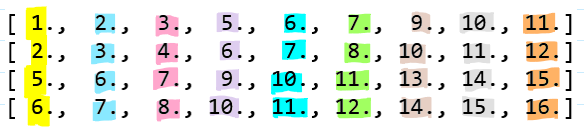
\includegraphics[height=1.5cm]{images/flatten.png}}\\
$\Downarrow$\\
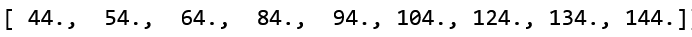
\includegraphics[height=0.45cm]{images/result.png}\\
$\Downarrow$\\
\vspace*{0.1cm}
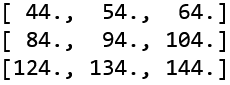
\includegraphics[height=1cm]{images/reshape.png}
\end{center}
\end{frame}

\begin{frame}
\frametitle{Backpropagation}
\begin{center}
Backpropagation is also a convolution!\\

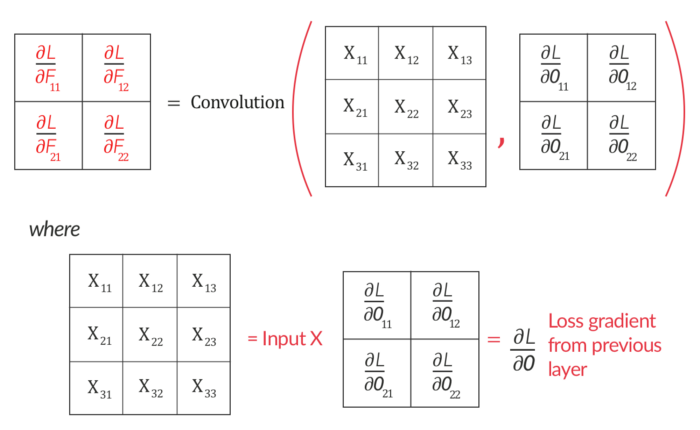
\includegraphics[height=6cm]{images/backprop.png}
\end{center}
\end{frame}

\begin{frame}
\frametitle{Backpropagation}
\begin{center}
Backpropagation is also a convolution!\\

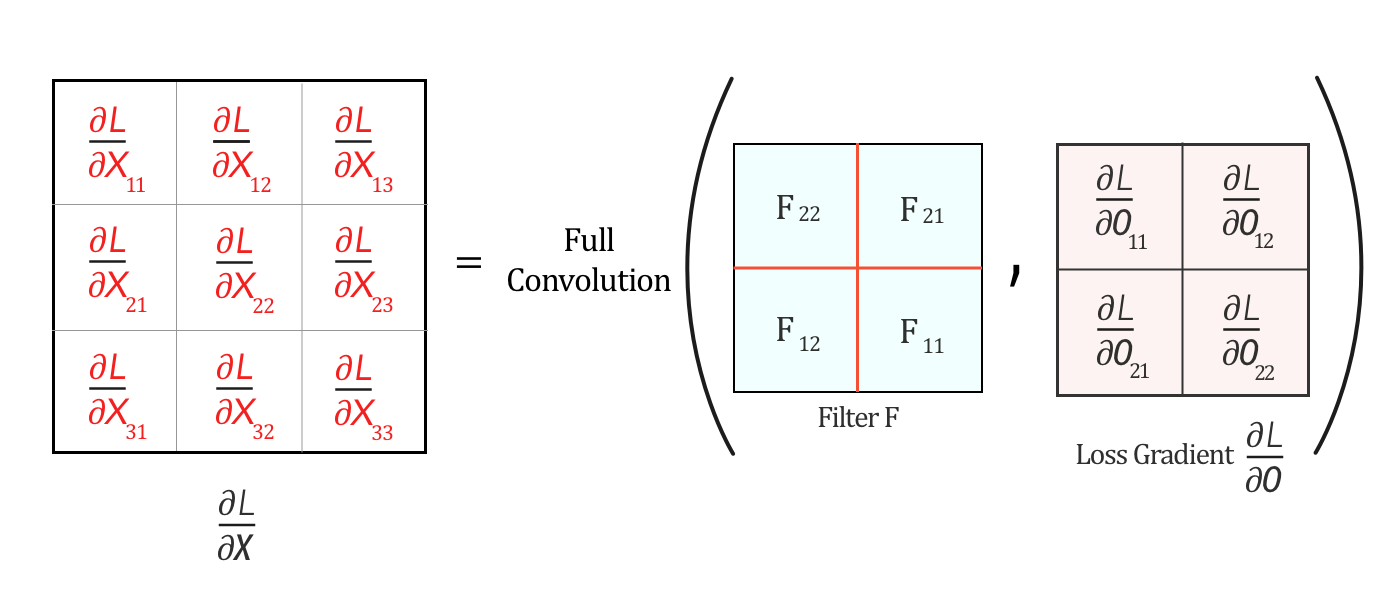
\includegraphics[height=4cm]{images/backprop2.png}
\end{center}
\end{frame}

\begin{frame}
\frametitle{Subsampling layer}
	\begin{center}
	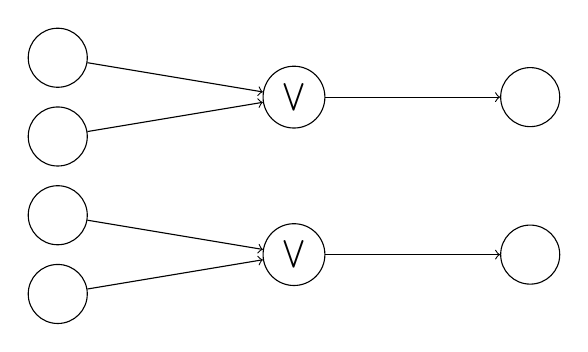
\begin{tikzpicture}
    \node[draw,circle,minimum size=0.75cm] at (3,3.15) (a1) {};
    \node[draw,circle,minimum size=0.75cm] at (3,2.15) (b1) {};
    \node[draw,circle,minimum size=0.75cm] at (3,1.15) (c1) {};
    \node[draw,circle,minimum size=0.75cm] at (3,0.15) (d1) {};

    \node[draw,circle,minimum size=0.75cm] at (6,2.65) (a2) {$\bigvee$};
    \node[draw,circle,minimum size=0.75cm] at (6,0.65) (b2) {$\bigvee$};

    \node[draw,circle,minimum size=0.75cm] at (9,2.65) (a3) {};
    \node[draw,circle,minimum size=0.75cm] at (9,0.65) (b3) {};

	\draw[->] (a1) -- (a2);
	\draw[->] (b1) -- (a2);
	\draw[->] (c1) -- (b2);
	\draw[->] (d1) -- (b2);

	\draw[->] (a2) -- (a3);
	\draw[->] (b2) -- (b3);
	\end{tikzpicture}
	\end{center}
\begin{itemize}
\item Reduce number of neurons in layers ($\approx$ increase receptive fields)
\item {\color{red} Max-pooling}: take the {\color{red} maximum} over the inputs
  \[o=\max_ix_i\]
\item Error only propagated to the maximum incoming neuron!
\end{itemize}
\end{frame}

\begin{frame}
\frametitle{Convolutional neural network}
\centerline{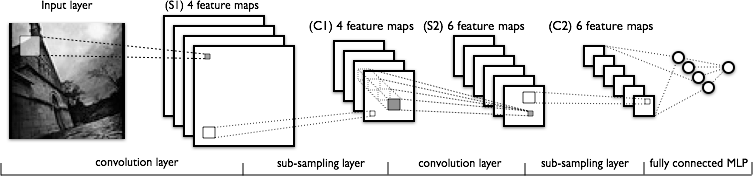
\includegraphics[height=3cm]{images/mylenet.png}}
\begin{itemize}
\item Combine convolutional and subsampling layers
\item Often include fully connected layers at the end
\end{itemize}
\end{frame}

\begin{frame}
\frametitle{Other uses of convolutional networks}
\centerline{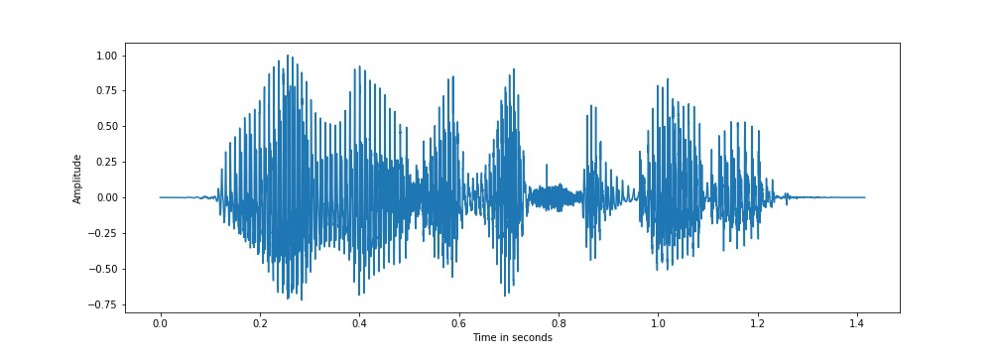
\includegraphics[height=4cm]{images/speech.png}}
\begin{itemize}
\item Somewhat surprisingly, CNNs work well for other inputs
\item Applications include {\color{red} speech recognition} and {\color{blue} natural language analysis}
\end{itemize}
\end{frame}

\end{document}
